\documentclass[hyperref={pdfpagelabels=false}]{beamer}

\def\pgfsysdriver{pgfsys-dvipdfmx.def}

\usepackage{multirow}
\usepackage{amsthm}
\usepackage{graphicx}
\usepackage{tabulary}
\usepackage{amssymb}
\usepackage{pgf}
\usepackage{clrscode3e}
\usepackage{tikz}
\usepackage{xspace}
\usepackage{xmpmulti}
\usepackage{array}
\usepackage[absolute,overlay]{textpos}
\usepackage{forloop}
\usepackage{subfigure}

\usetikzlibrary{shapes,arrows,decorations.pathmorphing,backgrounds,positioning,fit}
\usepgfmodule{plot}

\setbeamercovered{transparent}

\usecolortheme{rose}

\setbeamerfont{frametitle}{series=\bfseries}
\setbeamercolor*{title}{fg=white}
\setbeamercolor*{author}{fg=white}
\setbeamercolor*{institute}{fg=white}
\setbeamercolor*{date}{fg=white}
\setbeamerfont{title}{series=\bfseries,size=\huge}
\setbeamerfont{author}{series=\bfseries}

\setbeamercolor{postit}{fg=black,bg=example text.fg!75!black!10!bg}

\useinnertheme{default}
\setbeamertemplate{navigation symbols}{}

\title{Paths, Trees, and Flowers}
\author{Jack Edmonds}
\institute{ETH Zurich -- Distributed Computing Group -- www.disco.ethz.ch}

\begin{document}

%---------------------slide--------------------%
{
\usebackgroundtemplate{
\includegraphics[width=\paperwidth]{figures/bg}}
\begin{frame}
	\begin{textblock*}{\paperwidth}[0,0](0cm,1cm)
		\begin{center}
			\usebeamercolor[fg]{title}
			\textbf{\huge \inserttitle}
		\end{center}
		\usebeamercolor[fg]{normal text}
	\end{textblock*}
	\begin{textblock*}{\paperwidth}[0,0](-0.5cm,7.4cm)
		\flushright
		\color{white}
		\itshape \insertauthor
		\usebeamercolor[fg]{normal text}
	\end{textblock*}
	\begin{textblock*}{\paperwidth}[0,1](0.2cm,9.4cm)
		\flushleft
 		\usebeamercolor[fg]{institute}
		\tiny \itshape \insertinstitute
		\usebeamercolor[fg]{normal text}
	\end{textblock*}
\end{frame}
}

%---------------------slide--------------------%
\frame{\tableofcontents}

%---------------------slide--------------------%
\frame
{
	\frametitle{Work scheduling}
	Schedule workers in pairs. What is the optimal assignment?
	\begin{figure}[htb]
	\centering
	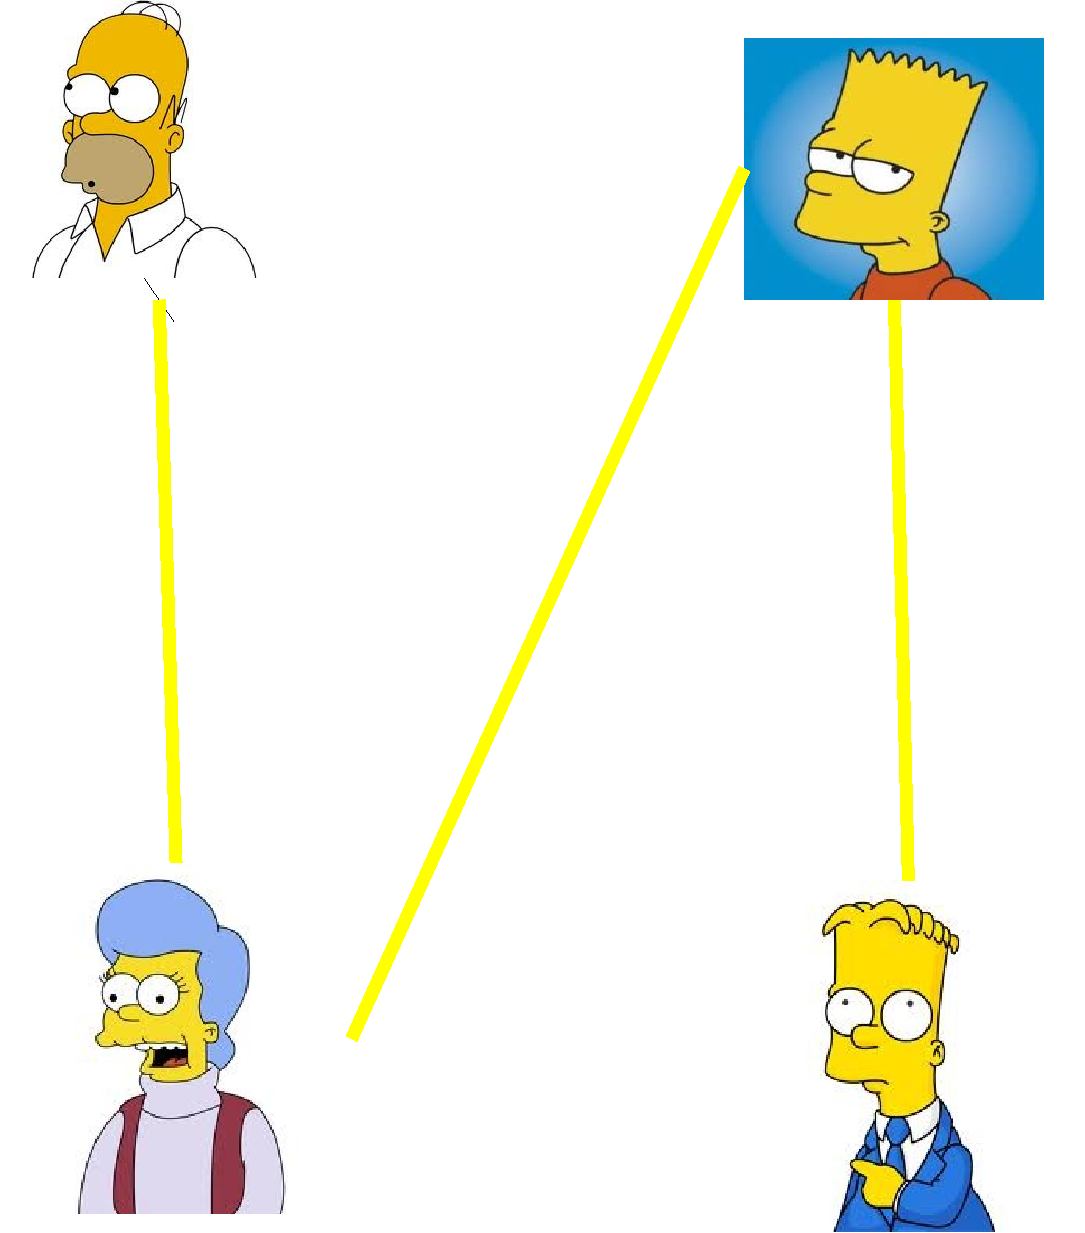
\includegraphics[width=0.6\textwidth]{figures/example.pdf}
	\end{figure}
}

%---------------------slide--------------------%
\section{Introduction and background}
\frame
{
	\frametitle{Matching}
	
	\uncover<1>{
	\begin{description}
		\item[Matching in a graph] is a set of edges, no two of which meet at a common vertex.
	\end{description}
	
	\begin{center}
		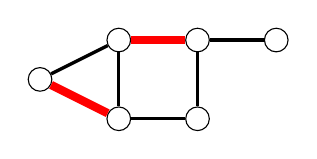
\begin{tikzpicture}[scale=0.5]
			\tikzstyle{Flower}	= [circle, fill=white, minimum size=4mm, inner sep=0pt]
			\tikzstyle{Vertex} 	= [circle, draw, solid,  fill=white, minimum size=3mm, inner sep=0pt]
			\tikzstyle{OUT}		= [fill = white]
			\tikzstyle{IN}		= [fill = black]
			\tikzstyle{Exposed}	= [dashed, blue, OUT]
			\tikzstyle{MC}		= [line width=3pt]
			\tikzstyle{NM}		= [very thick, black]
			
			\foreach \x/\y in {0/1, 2/0, 2/2, 4/0, 4/2, 6/2}
				\node (v\x\y) at (\x, \y) [Vertex] {};
			
			\foreach \a/\b/\c/\d in {0/1/2/2, 2/2/2/0, 2/0/4/0, 4/0/4/2, 4/2/6/2}
				\draw [-] (v\a\b) to (v\c\d) [NM];
			\foreach \a/\b/\c/\d in {0/1/2/0, 2/2/4/2}
				\draw [-] (v\a\b) to (v\c\d) [MC][red];
		\end{tikzpicture}
	\end{center}
	}
	%\pause
	\uncover<2>{
	\begin{description}
		\item[Maximum matching] is a matching of maximum cardinality.
	\end{description}
	
	\begin{center}
		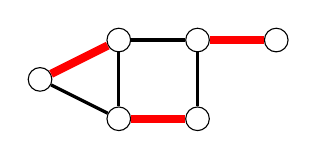
\begin{tikzpicture}[scale=0.5]
			\tikzstyle{Flower}	= [circle, fill=white, minimum size=4mm, inner sep=0pt]
			\tikzstyle{Vertex} 	= [circle, draw, solid,  fill=white, minimum size=3mm, inner sep=0pt]
			\tikzstyle{OUT}		= [fill = white]
			\tikzstyle{IN}		= [fill = black]
			\tikzstyle{Exposed}	= [dashed, blue, OUT]
			\tikzstyle{MC}		= [line width=3pt]
			\tikzstyle{NM}		= [very thick, black]
			
			\foreach \x/\y in {0/1, 2/0, 2/2, 4/0, 4/2, 6/2}
				\node (v\x\y) at (\x, \y) [Vertex] {};
			
			\foreach \a/\b/\c/\d in {0/1/2/0, 2/2/2/0, 2/2/4/2, 4/0/4/2}
				\draw [-] (v\a\b) to (v\c\d) [NM];
			\foreach \a/\b/\c/\d in {0/1/2/2, 2/0/4/0, 4/2/6/2}
				\draw [-] (v\a\b) to (v\c\d) [MC][red];
		\end{tikzpicture}
	\end{center}}
}

%---------------------slide--------------------%
\frame
{
	\frametitle{Exposed vertex}
	\begin{description}
		\item[Exposed(free) vertex] is a vertex that is not incident with any edge in $M$
	\end{description}
	
	\begin{center}
		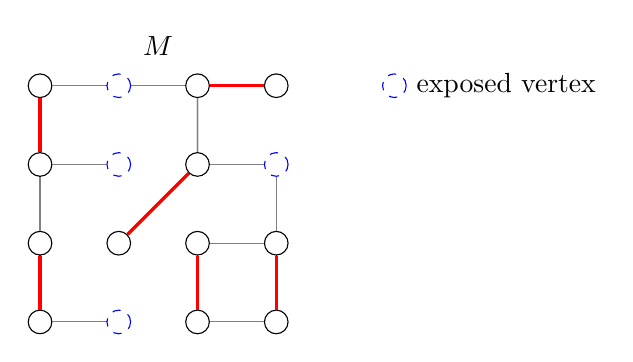
\begin{tikzpicture}
			\tikzstyle{Flower}	= [circle, fill=white, minimum size=4mm, inner sep=0pt]
			\tikzstyle{Vertex} 	= [circle, draw, solid,  fill=white, minimum size=3mm, inner sep=0pt]
			\tikzstyle{OUT}		= [fill = white]
			\tikzstyle{IN}		= [fill = black]
			\tikzstyle{Exposed}	= [dashed, blue, OUT]
			\tikzstyle{MC}		= [very thick, black]
			\tikzstyle{NM}		= [gray]
			
			
			\draw (2,0) -- (3,0) -- (3,1) -- (2,1) -- cycle;
			\draw (1,1) -- (2,2) -- (2,3) -- (3,3);
			\draw (1,0) -- (0,0) -- (0,1) -- (0,2) -- (0,3) -- (1,3);
			
			\draw (1.5, 3.5) node {$M$};
			\foreach \x/\y in {0/0, 2/0, 3/0, 0/1, 1/1, 2/1, 3/1, 0/2, 2/2, 0/3, 2/3, 3/3}
				\node (v\x\y) at (\x, \y) [Vertex] {};
			\foreach \x/\y in {1/0, 1/2, 3/2, 1/3}
				\node (v\x\y) at (\x, \y) [Vertex][Exposed] {};
			\foreach \a/\b/\c/\d in {0/0/1/0, 0/2/1/2, 2/0/3/0, 2/1/3/1, 2/2/3/2, 2/2/2/3, 2/0/2/1, 3/0/3/1, 0/1/0/2, 1/1/2/2, 0/3/1/3, 2/3/3/3, 1/3/2/3, 3/1/3/2, 0/0/0/1, 0/2/0/3}
				\draw [-] (v\a\b) to (v\c\d) [NM];
			\foreach \a/\b/\c/\d in {2/0/2/1, 3/0/3/1, 0/0/0/1, 1/1/2/2, 0/2/0/3, 2/3/3/3}
				\draw [-] (v\a\b) to (v\c\d) [MC][red];
			
			\node at (4.5, 3) [Vertex][Exposed][label=right:exposed vertex] {};
		\end{tikzpicture}
	\end{center}
}

%---------------------slide--------------------%
\frame
{
	\frametitle{Alternating path}
	\begin{description}
		\item[Alternating path] is a path whose edges are alternately in $M$ and $\overline{M}$
	\end{description}
	
	\begin{center}
		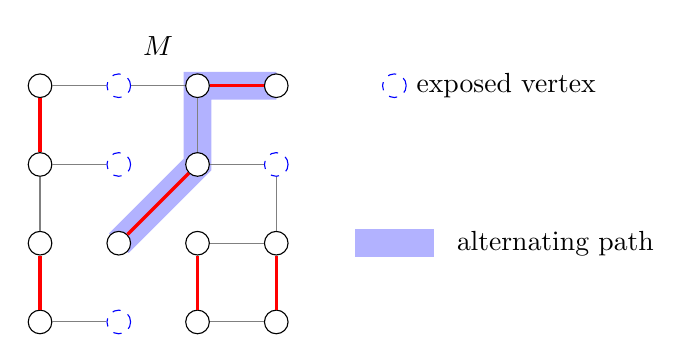
\begin{tikzpicture}
			\tikzstyle{Flower}	= [circle, fill=white, minimum size=4mm, inner sep=0pt]
			\tikzstyle{Vertex} 	= [circle, draw, solid,  fill=white, minimum size=3mm, inner sep=0pt]
			\tikzstyle{OUT}		= [fill = white]
			\tikzstyle{IN}		= [fill = black]
			\tikzstyle{Exposed}	= [dashed, blue, OUT]
			\tikzstyle{MC}		= [very thick, black]
			\tikzstyle{NM}		= [gray]
			
			\draw (1,1) -- (2,2) -- (2,3) -- (3,3) [line width=10pt, blue, opacity=0.3];
			
			\draw (1.5, 3.5) node {$M$};
			\foreach \x/\y in {0/0, 2/0, 3/0, 0/1, 1/1, 2/1, 3/1, 0/2, 2/2, 0/3, 2/3, 3/3}
				\node (v\x\y) at (\x, \y) [Vertex] {};
			\foreach \x/\y in {1/0, 1/2, 3/2, 1/3}
				\node (v\x\y) at (\x, \y) [Vertex][Exposed] {};
			\foreach \a/\b/\c/\d in {0/0/1/0, 0/2/1/2, 2/0/3/0, 2/1/3/1, 2/2/3/2, 2/2/2/3, 2/0/2/1, 3/0/3/1, 0/1/0/2, 1/1/2/2, 0/3/1/3, 2/3/3/3, 1/3/2/3, 3/1/3/2, 0/0/0/1, 0/2/0/3}
				\draw [-] (v\a\b) to (v\c\d) [NM];
			\foreach \a/\b/\c/\d in {2/0/2/1, 3/0/3/1, 0/0/0/1, 1/1/2/2, 0/2/0/3, 2/3/3/3}
				\draw [-] (v\a\b) to (v\c\d) [MC][red];
			
			\node at (4.5, 3) [Vertex][Exposed][label=right:exposed vertex] {};
			\draw (4,1) -- (5,1) [line width=10pt, blue, opacity=0.3] node [right, black, opacity=1]{alternating path};
		\end{tikzpicture}
	\end{center}
}

%---------------------slide--------------------%
\frame
{
	\frametitle{Different kinds of alternating path}
	
	\uncover<1>{
	\noindent An alternating path between two matched vertices\\
	\begin{center}
	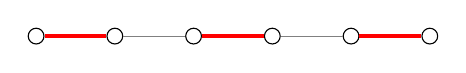
\begin{tikzpicture}
		\tikzstyle{Flower}	= [circle, fill=white, minimum size=2mm, inner sep=0pt]
		\tikzstyle{Vertex} 	= [circle, draw, solid,  fill=white, minimum size=2mm, inner sep=0pt]
		\tikzstyle{OUT}		= [fill = white]
		\tikzstyle{IN}		= [fill = black]
		\tikzstyle{Exposed}	= [dashed, OUT]
		\tikzstyle{MC}		= [very thick, red]
		\tikzstyle{NM}		= [gray]
		
		\node (v0) at (0,0) [Vertex] {};
		\node (v1) at (1,0) [Vertex] {};
		\node (v2) at (2,0) [Vertex] {};
		\node (v3) at (3,0) [Vertex] {};
		\node (v4) at (4,0) [Vertex] {};
		\node (v5) at (5,0) [Vertex] {};
		
		\draw [-] (v0) to (v1) [MC];
		\draw [-] (v1) to (v2) [NM];
		\draw [-] (v2) to (v3) [MC];
		\draw [-] (v3) to (v4) [NM];
		\draw [-] (v4) to (v5) [MC];
	\end{tikzpicture}
	\end{center}}
	
	\uncover<2>{
	\noindent An alternating path between two exposed vertices\\
	\begin{center}
	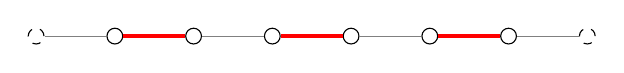
\begin{tikzpicture}
		\tikzstyle{Flower}	= [circle, fill=white, minimum size=2mm, inner sep=0pt]
		\tikzstyle{Vertex} 	= [circle, draw, solid,  fill=white, minimum size=2mm, inner sep=0pt]
		\tikzstyle{OUT}		= [fill = white]
		\tikzstyle{IN}		= [fill = black]
		\tikzstyle{Exposed}	= [dashed, OUT]
		\tikzstyle{MC}		= [very thick, red]
		\tikzstyle{NM}		= [gray]
		
		\node (v0) at (0,0) [Vertex][Exposed] {};
		\node (v1) at (1,0) [Vertex] {};
		\node (v2) at (2,0) [Vertex] {};
		\node (v3) at (3,0) [Vertex] {};
		\node (v4) at (4,0) [Vertex] {};
		\node (v5) at (5,0) [Vertex] {};
		\node (v6) at (6,0) [Vertex] {};
		\node (v7) at (7,0) [Vertex][Exposed] {};
		
		\draw [-] (v0) to (v1) [NM];
		\draw [-] (v1) to (v2) [MC];
		\draw [-] (v2) to (v3) [NM];
		\draw [-] (v3) to (v4) [MC];
		\draw [-] (v4) to (v5) [NM];
		\draw [-] (v5) to (v6) [MC];
		\draw [-] (v6) to (v7) [NM];
	\end{tikzpicture}
	\end{center}}
	
	\uncover<3>{
	\noindent An alternating path between a matched vertex and an exposed vertex\\
	\begin{center}
	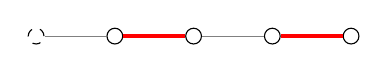
\begin{tikzpicture}
		\tikzstyle{Flower}	= [circle, fill=white, minimum size=2mm, inner sep=0pt]
		\tikzstyle{Vertex} 	= [circle, draw, solid,  fill=white, minimum size=2mm, inner sep=0pt]
		\tikzstyle{OUT}		= [fill = white]
		\tikzstyle{IN}		= [fill = black]
		\tikzstyle{Exposed}	= [dashed, OUT]
		\tikzstyle{MC}		= [very thick, red]
		\tikzstyle{NM}		= [gray]
		
		\node (v0) at (0,0) [Vertex][Exposed] {};
		\node (v1) at (1,0) [Vertex] {};
		\node (v2) at (2,0) [Vertex] {};
		\node (v3) at (3,0) [Vertex] {};
		\node (v4) at (4,0) [Vertex] {};
		
		\draw [-] (v0) to (v1) [NM];
		\draw [-] (v1) to (v2) [MC];
		\draw [-] (v2) to (v3) [NM];
		\draw [-] (v3) to (v4) [MC];
	\end{tikzpicture}
	\end{center}}
	
	\uncover<4>{
	\noindent An alternating cycle\\
	\begin{center}
	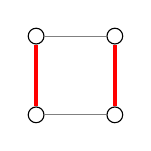
\begin{tikzpicture}
		\tikzstyle{Flower}	= [circle, fill=white, minimum size=2mm, inner sep=0pt]
		\tikzstyle{Vertex} 	= [circle, draw, solid,  fill=white, minimum size=2mm, inner sep=0pt]
		\tikzstyle{OUT}		= [fill = white]
		\tikzstyle{IN}		= [fill = black]
		\tikzstyle{Exposed}	= [dashed, OUT]
		\tikzstyle{MC}		= [very thick, red]
		\tikzstyle{NM}		= [gray]
		
		\node (v0) at (0,0) [Vertex] {};
		\node (v1) at (1,0) [Vertex] {};
		\node (v2) at (1,1) [Vertex] {};
		\node (v3) at (0,1) [Vertex] {};
		
		\draw [-] (v0) to (v1) [NM];
		\draw [-] (v1) to (v2) [MC];
		\draw [-] (v2) to (v3) [NM];
		\draw [-] (v3) to (v0) [MC];
	\end{tikzpicture}
	\end{center}}
}

%---------------------slide--------------------%
\frame
{
	\frametitle{Augmenting path}
	\begin{description}
		\item[Augmenting path] is a simple alternating path between exposed vertices
	\end{description}
	
	\begin{center}
		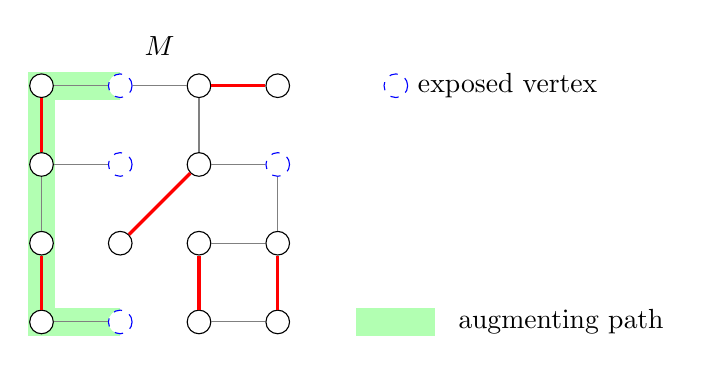
\begin{tikzpicture}
			\tikzstyle{Flower}	= [circle, fill=white, minimum size=4mm, inner sep=0pt]
			\tikzstyle{Vertex} 	= [circle, draw, solid,  fill=white, minimum size=3mm, inner sep=0pt]
			\tikzstyle{OUT}		= [fill = white]
			\tikzstyle{IN}		= [fill = black]
			\tikzstyle{Exposed}	= [dashed, blue, OUT]
			\tikzstyle{MC}		= [very thick, black]
			\tikzstyle{NM}		= [gray]
			
			\draw (1,0) -- (0,0) -- (0,1) -- (0,2) -- (0,3) -- (1,3) [line width=10pt, green, opacity=0.3];
			
			\draw (1.5, 3.5) node {$M$};
			\foreach \x/\y in {0/0, 2/0, 3/0, 0/1, 1/1, 2/1, 3/1, 0/2, 2/2, 0/3, 2/3, 3/3}
				\node (v\x\y) at (\x, \y) [Vertex] {};
			\foreach \x/\y in {1/0, 1/2, 3/2, 1/3}
				\node (v\x\y) at (\x, \y) [Vertex][Exposed] {};
			\foreach \a/\b/\c/\d in {0/0/1/0, 0/2/1/2, 2/0/3/0, 2/1/3/1, 2/2/3/2, 2/2/2/3, 2/0/2/1, 3/0/3/1, 0/1/0/2, 1/1/2/2, 0/3/1/3, 2/3/3/3, 1/3/2/3, 3/1/3/2, 0/0/0/1, 0/2/0/3}
				\draw [-] (v\a\b) to (v\c\d) [NM];
			\foreach \a/\b/\c/\d in {2/0/2/1, 3/0/3/1, 0/0/0/1, 1/1/2/2, 0/2/0/3, 2/3/3/3}
				\draw [-] (v\a\b) to (v\c\d) [MC][red];
			
			\node at (4.5, 3) [Vertex][Exposed][label=right:exposed vertex] {};
			\draw (4,0) -- (5,0) [line width=10pt, green, opacity=0.3] node [right, black, opacity=1]{augmenting path};
		\end{tikzpicture}
	\end{center}
}

%---------------------slide--------------------%
\frame
{
	\frametitle{Symmetric difference}
	\begin{description}
		\item[Symmetric difference] of two sets $D$ and $E$ is defined as $D \oplus E = (D - E) \cup (E - D)$
	\end{description}
	
	\begin{center}
	\begin{figure}[h]
		\hfill
		\centering
		\begin{minipage}[c]{.45\textwidth}
		\centering
		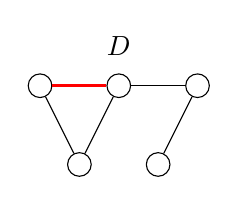
\begin{tikzpicture}
			\tikzstyle{Flower}	= [circle, fill=white, minimum size=4mm, inner sep=0pt]
			\tikzstyle{Vertex} 	= [circle, draw, solid,  fill=white, minimum size=3mm, inner sep=0pt]
			\tikzstyle{OUT}		= [fill = white]
			\tikzstyle{IN}		= [fill = black]
			\tikzstyle{Exposed}	= [dashed, blue, OUT]
			\tikzstyle{MC}		= [very thick]
			\tikzstyle{NM}		= [black]
			
			\draw (1, 1.5) node {$D$};
			\node (v1) at (0, 1) [Vertex] {};
			\node (v2) at (0.5, 0) [Vertex] {};
			\node (v3) at (1, 1) [Vertex] {};
			\node (v4) at (1.5, 0) [Vertex] {};
			\node (v5) at (2, 1) [Vertex] {};
			
			\draw [-] (v1) to (v2) [NM];
			\draw [-] (v2) to (v3) [NM];
			\draw [-] (v3) to (v5) [NM];
			\draw [-] (v4) to (v5) [NM];
			
			\draw [-] (v1) to (v3) [MC][red];
		\end{tikzpicture}
		\end{minipage}
		\hfill
		\centering
		\begin{minipage}[c]{.45\textwidth}
		\centering
		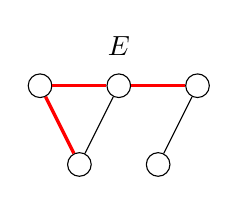
\begin{tikzpicture}
			\tikzstyle{Flower}	= [circle, fill=white, minimum size=4mm, inner sep=0pt]
			\tikzstyle{Vertex} 	= [circle, draw, solid,  fill=white, minimum size=3mm, inner sep=0pt]
			\tikzstyle{OUT}		= [fill = white]
			\tikzstyle{IN}		= [fill = black]
			\tikzstyle{Exposed}	= [dashed, blue, OUT]
			\tikzstyle{MC}		= [very thick]
			\tikzstyle{NM}		= [black]
			
			\draw (1, 1.5) node {$E$};
			\node (v1) at (0, 1) [Vertex] {};
			\node (v2) at (0.5, 0) [Vertex] {};
			\node (v3) at (1, 1) [Vertex] {};
			\node (v4) at (1.5, 0) [Vertex] {};
			\node (v5) at (2, 1) [Vertex] {};
			
			\draw [-] (v2) to (v3) [NM];
			\draw [-] (v4) to (v5) [NM];
			
			\draw [-] (v1) to (v3) [MC][red];
			\draw [-] (v1) to (v2) [MC][red];
			\draw [-] (v3) to (v5) [MC][red];
		\end{tikzpicture}
		\end{minipage}
		\hfill
	\end{figure}
	\end{center}
	
	\begin{center}
	\begin{figure}[h]
		\centering
		\begin{minipage}[c]{.45\textwidth}
		\centering
		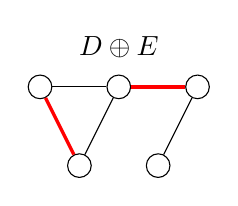
\begin{tikzpicture}
			\tikzstyle{Flower}	= [circle, fill=white, minimum size=4mm, inner sep=0pt]
			\tikzstyle{Vertex} 	= [circle, draw, solid,  fill=white, minimum size=3mm, inner sep=0pt]
			\tikzstyle{OUT}		= [fill = white]
			\tikzstyle{IN}		= [fill = black]
			\tikzstyle{Exposed}	= [dashed, blue, OUT]
			\tikzstyle{MC}		= [very thick]
			\tikzstyle{NM}		= [black]
			
			\draw (1, 1.5) node {$D \oplus E$};
			\node (v1) at (0, 1) [Vertex] {};
			\node (v2) at (0.5, 0) [Vertex] {};
			\node (v3) at (1, 1) [Vertex] {};
			\node (v4) at (1.5, 0) [Vertex] {};
			\node (v5) at (2, 1) [Vertex] {};
			
			\draw [-] (v2) to (v3) [NM];
			\draw [-] (v4) to (v5) [NM];
			\draw [-] (v1) to (v3) [NM];
			
			\draw [-] (v1) to (v2) [MC][red];
			\draw [-] (v3) to (v5) [MC][red];
		\end{tikzpicture}
		\end{minipage}
	\end{figure}
	\end{center}
}

%---------------------slide--------------------%
\frame
{
	\frametitle{Alternating path}
	
	\begin{beamercolorbox}[sep=1em,wd=11cm]{postit}
		For any two matchings $M_{1}$ and $M_{2}$ in graph $G$, the components of the graph formed by $M_{1} \oplus M_{2}$ are paths and circuits which are alternating for $M_{1}$ and $M_{2}$. Each path end-point is exposed for either $M_{1}$ or $M_{2}$.
	\end{beamercolorbox}
	
	\begin{center}
	\begin{figure}[h]
		\hfill
		\centering
		\begin{minipage}[c]{.45\textwidth}
		\centering
		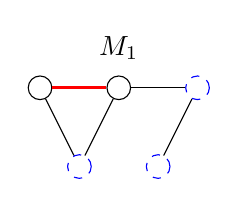
\begin{tikzpicture}
			\tikzstyle{Flower}	= [circle, fill=white, minimum size=4mm, inner sep=0pt]
			\tikzstyle{Vertex} 	= [circle, draw, solid,  fill=white, minimum size=3mm, inner sep=0pt]
			\tikzstyle{OUT}		= [fill = white]
			\tikzstyle{IN}		= [fill = black]
			\tikzstyle{Exposed1}	= [dashed, blue, OUT]
			\tikzstyle{MC}		= [very thick]
			\tikzstyle{NM}		= [black]
			
			\draw (1, 1.5) node {$M_{1}$};
			\node (v1) at (0, 1) [Vertex] {};
			\node (v2) at (0.5, 0) [Vertex][Exposed1] {};
			\node (v3) at (1, 1) [Vertex] {};
			\node (v4) at (1.5, 0) [Vertex][Exposed1] {};
			\node (v5) at (2, 1) [Vertex][Exposed1] {};
			
			\draw [-] (v1) to (v2) [NM];
			\draw [-] (v2) to (v3) [NM];
			\draw [-] (v3) to (v5) [NM];
			\draw [-] (v4) to (v5) [NM];
			
			\draw [-] (v1) to (v3) [MC][red];
		\end{tikzpicture}
		\end{minipage}
		\hfill
		\centering
		\begin{minipage}[c]{.45\textwidth}
		\centering
		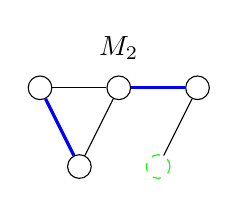
\begin{tikzpicture}
			\tikzstyle{Flower}	= [circle, fill=white, minimum size=4mm, inner sep=0pt]
			\tikzstyle{Vertex} 	= [circle, draw, solid,  fill=white, minimum size=3mm, inner sep=0pt]
			\tikzstyle{OUT}		= [fill = white]
			\tikzstyle{IN}		= [fill = black]
			\tikzstyle{Exposed2}	= [dashed, green, OUT]
			\tikzstyle{MC}		= [very thick]
			\tikzstyle{NM}		= [black]
			
			\draw (1, 1.5) node {$M_{2}$};
			\node (v1) at (0, 1) [Vertex] {};
			\node (v2) at (0.5, 0) [Vertex] {};
			\node (v3) at (1, 1) [Vertex] {};
			\node (v4) at (1.5, 0) [Vertex][Exposed2] {};
			\node (v5) at (2, 1) [Vertex] {};
			
			\draw [-] (v2) to (v3) [NM];
			\draw [-] (v4) to (v5) [NM];
			\draw [-] (v1) to (v3) [NM];
			
			\draw [-] (v1) to (v2) [MC][blue];
			\draw [-] (v3) to (v5) [MC][blue];
		\end{tikzpicture}
		\end{minipage}
		\hfill
	\end{figure}
	\end{center}
	
	\begin{center}
	\begin{figure}[h]
		\centering
		\begin{minipage}[c]{.45\textwidth}
		\centering
		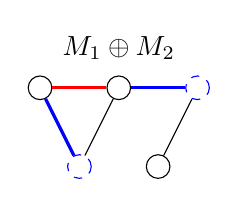
\begin{tikzpicture}
			\tikzstyle{Flower}	= [circle, fill=white, minimum size=4mm, inner sep=0pt]
			\tikzstyle{Vertex} 	= [circle, draw, solid,  fill=white, minimum size=3mm, inner sep=0pt]
			\tikzstyle{OUT}		= [fill = white]
			\tikzstyle{IN}		= [fill = black]
			\tikzstyle{Exposed1}	= [dashed, blue, OUT]
			\tikzstyle{Exposed2}	= [dashed, green, OUT]
			\tikzstyle{MC}		= [very thick]
			\tikzstyle{NM}		= [black]
			
			\draw (1, 1.5) node {$M_{1} \oplus M_{2}$};
			\node (v1) at (0, 1) [Vertex] {};
			\node (v2) at (0.5, 0) [Vertex][Exposed1] {};
			\node (v3) at (1, 1) [Vertex] {};
			\node (v4) at (1.5, 0) [Vertex] {};
			\node (v5) at (2, 1) [Vertex][Exposed1] {};
			
			\draw [-] (v2) to (v3) [NM];
			\draw [-] (v4) to (v5) [NM];
			
			\draw [-] (v1) to (v2) [MC][blue];
			\draw [-] (v1) to (v3) [MC][red];
			\draw [-] (v3) to (v5) [MC][blue];
		\end{tikzpicture}
		\end{minipage}
	\end{figure}
	\end{center}
}

%---------------------slide--------------------%
\frame
{
	\frametitle{Augmenting path}
	\begin{beamercolorbox}[sep=1em,wd=11cm]{postit}
		$A$ is an augmenting path in $(G, M)$ . $M \oplus A$ is a matching of $G$ larger than $M$ by one.
	\end{beamercolorbox}
	
	\begin{center}
	\begin{figure}
		\hfill
		\centering
		\begin{minipage}[c]{.45\textwidth}
		\centering
		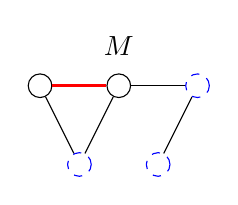
\begin{tikzpicture}
			\tikzstyle{Flower}	= [circle, fill=white, minimum size=4mm, inner sep=0pt]
			\tikzstyle{Vertex} 	= [circle, draw, solid,  fill=white, minimum size=3mm, inner sep=0pt]
			\tikzstyle{OUT}		= [fill = white]
			\tikzstyle{IN}		= [fill = black]
			\tikzstyle{Exposed1}	= [dashed, blue, OUT]
			\tikzstyle{MC}		= [very thick]
			\tikzstyle{NM}		= [black]
			
			\draw (1, 1.5) node {$M$};
			\node (v1) at (0, 1) [Vertex] {};
			\node (v2) at (0.5, 0) [Vertex][Exposed1] {};
			\node (v3) at (1, 1) [Vertex] {};
			\node (v4) at (1.5, 0) [Vertex][Exposed1] {};
			\node (v5) at (2, 1) [Vertex][Exposed1] {};
			
			\draw [-] (v1) to (v2) [NM];
			\draw [-] (v2) to (v3) [NM];
			\draw [-] (v3) to (v5) [NM];
			\draw [-] (v4) to (v5) [NM];
			
			\draw [-] (v1) to (v3) [MC][red];
		\end{tikzpicture}
		\end{minipage}
		\hfill
		\centering
		\begin{minipage}[c]{.45\textwidth}
		\centering
		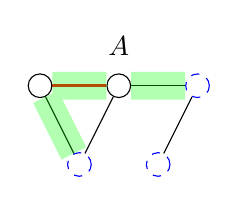
\begin{tikzpicture}
			\tikzstyle{Flower}	= [circle, fill=white, minimum size=4mm, inner sep=0pt]
			\tikzstyle{Vertex} 	= [circle, draw, solid,  fill=white, minimum size=3mm, inner sep=0pt]
			\tikzstyle{OUT}		= [fill = white]
			\tikzstyle{IN}		= [fill = black]
			\tikzstyle{Exposed1}	= [dashed, blue, OUT]
			\tikzstyle{MC}		= [very thick]
			\tikzstyle{NM}		= [black]
			
			\draw (1, 1.5) node {$A$};
			\node (v1) at (0, 1) [Vertex] {};
			\node (v2) at (0.5, 0) [Vertex][Exposed1] {};
			\node (v3) at (1, 1) [Vertex] {};
			\node (v4) at (1.5, 0) [Vertex][Exposed1] {};
			\node (v5) at (2, 1) [Vertex][Exposed1] {};
			
			\draw [-] (v1) to (v2) [NM];
			\draw [-] (v2) to (v3) [NM];
			\draw [-] (v3) to (v5) [NM];
			\draw [-] (v4) to (v5) [NM];
			
			\draw [-] (v1) to (v3) [MC][red];
			
			\draw (v2) -- (v1) -- (v3) -- (v5) [line width=10pt, green, opacity=0.3];
		\end{tikzpicture}
		\end{minipage}
		\hfill
	\end{figure}
	\end{center}
	
	\begin{center}
	\begin{figure}[h]
		\centering
		\begin{minipage}[c]{.45\textwidth}
		\centering
		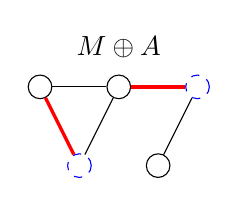
\begin{tikzpicture}
			\tikzstyle{Flower}	= [circle, fill=white, minimum size=4mm, inner sep=0pt]
			\tikzstyle{Vertex} 	= [circle, draw, solid,  fill=white, minimum size=3mm, inner sep=0pt]
			\tikzstyle{OUT}		= [fill = white]
			\tikzstyle{IN}		= [fill = black]
			\tikzstyle{Exposed1}	= [dashed, blue, OUT]
			\tikzstyle{Exposed2}	= [dashed, green, OUT]
			\tikzstyle{MC}		= [very thick]
			\tikzstyle{NM}		= [black]
			
			\draw (1, 1.5) node {$M \oplus A$};
			\node (v1) at (0, 1) [Vertex] {};
			\node (v2) at (0.5, 0) [Vertex][Exposed1] {};
			\node (v3) at (1, 1) [Vertex] {};
			\node (v4) at (1.5, 0) [Vertex] {};
			\node (v5) at (2, 1) [Vertex][Exposed1] {};
			
			\draw [-] (v2) to (v3) [NM];
			\draw [-] (v4) to (v5) [NM];
			\draw [-] (v1) to (v3) [NM];
			
			\draw [-] (v1) to (v2) [MC][red];
			\draw [-] (v3) to (v5) [MC][red];
		\end{tikzpicture}
		\end{minipage}
	\end{figure}
	\end{center}
}

%---------------------slide--------------------%
\frame
{
	\frametitle{Berge's theorem}
	
	\begin{block}{Theorem - Berge(1957)}
		$M$ is not a maximum matching if and only if there exists an augmenting path with respect to $M$
	\end{block}	
	
	\begin{itemize}
	{
		\item Proof:
		if $M_{2}$ is a larger matching than $M$, some component of graph $M \oplus M_{2}$ must contain more $M_{2}$ edges than $M$, such a component is an augmenting path for $(G, M)$.
	}
	\end{itemize}
	
	\begin{center}
	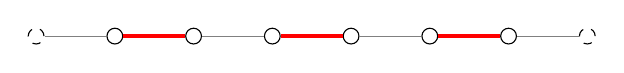
\begin{tikzpicture}
		\tikzstyle{Flower}	= [circle, fill=white, minimum size=2mm, inner sep=0pt]
		\tikzstyle{Vertex} 	= [circle, draw, solid,  fill=white, minimum size=2mm, inner sep=0pt]
		\tikzstyle{OUT}		= [fill = white]
		\tikzstyle{IN}		= [fill = black]
		\tikzstyle{Exposed}	= [dashed, OUT]
		\tikzstyle{MC}		= [very thick, red]
		\tikzstyle{NM}		= [gray]
		
		\node (v0) at (0,0) [Vertex][Exposed] {};
		\node (v1) at (1,0) [Vertex] {};
		\node (v2) at (2,0) [Vertex] {};
		\node (v3) at (3,0) [Vertex] {};
		\node (v4) at (4,0) [Vertex] {};
		\node (v5) at (5,0) [Vertex] {};
		\node (v6) at (6,0) [Vertex] {};
		\node (v7) at (7,0) [Vertex][Exposed] {};
		
		\draw [-] (v0) to (v1) [NM];
		\draw [-] (v1) to (v2) [MC];
		\draw [-] (v2) to (v3) [NM];
		\draw [-] (v3) to (v4) [MC];
		\draw [-] (v4) to (v5) [NM];
		\draw [-] (v5) to (v6) [MC];
		\draw [-] (v6) to (v7) [NM];
	\end{tikzpicture}
	\end{center}
}

%---------------------slide--------------------%
\frame
{
	\frametitle{Algorithm}

	\begin{codebox}
	\Procname{$\proc{Maximum-Matching}(G)$}
	\li $M \gets \emptyset$ 
	\li \Repeat
	\li		\If there is an augmenting path $P$ with respect to $M$ 
	\li			\Then		       
					$M \gets M \oplus P$
			\End
	\li	\Until there isn't an augmenting path with respect to $M$
	\li \Return $M$
	\end{codebox}
}

%---------------------slide--------------------%
\frame
{
	\frametitle{Bipartite Matching}
	Left circles represent boys, right diamonds represent girls, and edges are their preferences. We want to make maximum number of couples.
	\begin{center}
		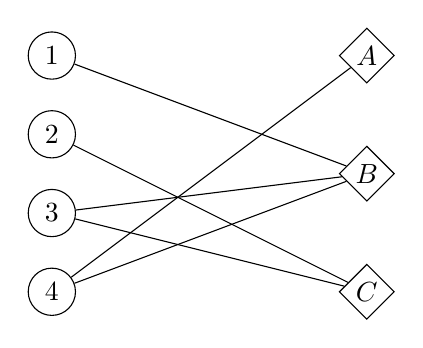
\begin{tikzpicture}
			\tikzstyle{Vertex} 	= [draw, solid,  fill=white, minimum size=6mm, inner sep=0pt]
			\tikzstyle{Exposed}	= []
			\tikzstyle{Boy}		= [circle]
			\tikzstyle{Girl}		= [diamond, minimum size=7mm]
			\tikzstyle{MC}		= [black]
			\tikzstyle{NM}		= [black]
			
			\node (b1) at (0,6) [Vertex][Boy][Exposed] {$1$};
			\node (b2) at (0,5) [Vertex][Boy][Exposed] {$2$};
			\node (b3) at (0,4) [Vertex][Boy] {$3$};
			\node (b4) at (0,3) [Vertex][Boy] {$4$};
			
			\node (ga) at (4,6.00) [Vertex][Girl][Exposed] {$A$};
			\node (gb) at (4,4.50) [Vertex][Girl] {$B$};
			\node (gc) at (4,3.00) [Vertex][Girl] {$C$};
			
			\draw [-] (b1) to (gb) [NM];
			\draw [-] (b2) to (gc) [NM];
			\draw [-] (b3) to (gb) [NM];
			\draw [-] (b3) to (gc) [MC];
			\draw [-] (b4) to (ga) [NM];
			\draw [-] (b4) to (gb) [MC];
		\end{tikzpicture}
	\end{center}
}

%---------------------slide--------------------%
\frame
{
	\frametitle{Find An Augmenting Path Using BFS}

	\begin{center}
	\begin{figure}[h]
	\hfill
		\centering
		\begin{minipage}[c]{.45\textwidth}
		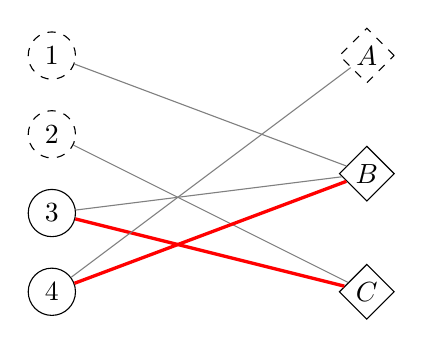
\begin{tikzpicture}
			\tikzstyle{Vertex} 	= [draw, solid,  fill=white, minimum size=6mm, inner sep=0pt]
			\tikzstyle{Exposed}	= [dashed]
			\tikzstyle{Boy}		= [circle]
			\tikzstyle{Girl}		= [diamond, minimum size=7mm]
			\tikzstyle{MC}		= [very thick, red]
			\tikzstyle{NM}		= [gray]
			
			\node (b1) at (0,6) [Vertex][Boy][Exposed] {$1$};
			\node (b2) at (0,5) [Vertex][Boy][Exposed] {$2$};
			\node (b3) at (0,4) [Vertex][Boy] {$3$};
			\node (b4) at (0,3) [Vertex][Boy] {$4$};
			
			\node (ga) at (4,6.00) [Vertex][Girl][Exposed] {$A$};
			\node (gb) at (4,4.50) [Vertex][Girl] {$B$};
			\node (gc) at (4,3.00) [Vertex][Girl] {$C$};
			
			\draw [-] (b1) to (gb) [NM];
			\draw [-] (b2) to (gc) [NM];
			\draw [-] (b3) to (gb) [NM];
			\draw [-] (b3) to (gc) [MC];
			\draw [-] (b4) to (ga) [NM];
			\draw [-] (b4) to (gb) [MC];
		\end{tikzpicture}
		\end{minipage}
	\hfill
		\centering
		\begin{minipage}[c]{.45\textwidth}
			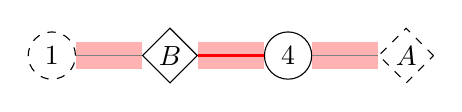
\begin{tikzpicture}
				\tikzstyle{Vertex} 	= [draw, solid,  fill=white, minimum size=6mm, inner sep=0pt]
				\tikzstyle{Exposed}	= [dashed]
				\tikzstyle{Boy}		= [circle]
				\tikzstyle{Girl}		= [diamond, minimum size=7mm]
				\tikzstyle{MC}		= [very thick, red]
				\tikzstyle{NM}		= [gray]
				
				\node (b1) at (0.0, 3) [Vertex][Boy][Exposed] {$1$};
					
				\node (gb) at (1.5, 3) [Vertex][Girl] {$B$};
				
				\node (b4) at (3.0, 3) [Vertex][Boy] {$4$};
					
				\node (ga) at (4.5, 3) [Vertex][Girl][Exposed] {$A$};
				
				\draw (b1) -- (gb) -- (b4) -- (ga) [line width=10pt, red, opacity=0.3];
					
				\draw [-] (b1) to (gb) [NM];
				\draw [-] (b4) to (ga) [NM];
				\draw [-] (b4) to (gb) [MC];
			\end{tikzpicture}
		\end{minipage}
	\hfill
	\end{figure}
	\end{center}
}

%---------------------slide--------------------%
\frame
{
	\frametitle{Find An Augmenting Path Using BFS}

	\begin{center}
	\begin{figure}[h]
	\hfill
		\centering
		\begin{minipage}[c]{.45\textwidth}
			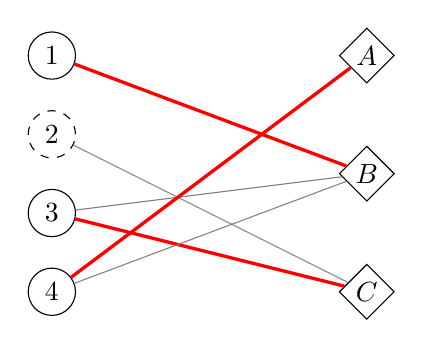
\begin{tikzpicture}
				\tikzstyle{Vertex} 	= [draw, solid,  fill=white, minimum size=6mm, inner sep=0pt]
				\tikzstyle{Exposed}	= [dashed]
				\tikzstyle{Boy}		= [circle]
				\tikzstyle{Girl}		= [diamond, minimum size=7mm]
				\tikzstyle{MC}		= [very thick, red]
				\tikzstyle{NM}		= [gray]
				
				\node (b1) at (0,6) [Vertex][Boy] {$1$};
				\node (b2) at (0,5) [Vertex][Boy][Exposed] {$2$};
				\node (b3) at (0,4) [Vertex][Boy] {$3$};
				\node (b4) at (0,3) [Vertex][Boy] {$4$};
				
				\node (ga) at (4,6.00) [Vertex][Girl] {$A$};
				\node (gb) at (4,4.50) [Vertex][Girl] {$B$};
				\node (gc) at (4,3.00) [Vertex][Girl] {$C$};
				
				\draw [-] (b1) to (gb) [MC];
				\draw [-] (b2) to (gc) [NM];
				\draw [-] (b3) to (gb) [NM];
				\draw [-] (b3) to (gc) [MC];
				\draw [-] (b4) to (ga) [MC];
				\draw [-] (b4) to (gb) [NM];
			\end{tikzpicture}
		\end{minipage}
	\hfill
		\centering
		\begin{minipage}[c]{.45\textwidth}
			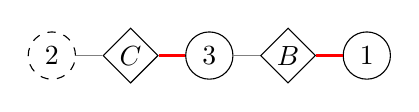
\begin{tikzpicture}
				\tikzstyle{Vertex} 	= [draw, solid,  fill=white, minimum size=6mm, inner sep=0pt]
				\tikzstyle{Exposed}	= [dashed]
				\tikzstyle{Boy}		= [circle]
				\tikzstyle{Girl}		= [diamond, minimum size=7mm]
				\tikzstyle{MC}		= [very thick, red]
				\tikzstyle{NM}		= [gray]
				
				\node (b2) at (0.0, 3) [Vertex][Boy][Exposed] {$2$};
					
				\node (gb) at (3, 3) [Vertex][Girl] {$B$};
				\node (gc) at (1.0, 3) [Vertex][Girl] {$C$};
				
				\node (b1) at (4.0, 3) [Vertex][Boy] {$1$};
				\node (b3) at (2.0, 3) [Vertex][Boy] {$3$};
														
				\draw [-] (b2) to (gc) [NM];
				\draw [-] (b3) to (gb) [NM];
				\draw [-] (b3) to (gc) [MC];
				\draw [-] (b1) to (gb) [MC];
			\end{tikzpicture}
		\end{minipage}
	\hfill
	\end{figure}
	\end{center}
}

%---------------------slide--------------------%
\frame
{
	\frametitle{Examples of BFS failure on non-bipartite graphs}
	\begin{itemize}
		\item Initial graph
	\end{itemize}
	{\mode<presentation>{\tiny}
	\begin{center}
	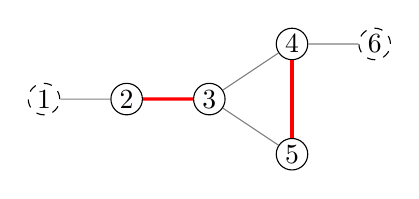
\begin{tikzpicture}[scale=0.7]
		\tikzstyle{Vertex} 	= [circle, draw, solid,  fill=white, minimum size=4mm, inner sep=0pt]
		\tikzstyle{Exposed}	= [dashed]
		\tikzstyle{MC}		= [very thick, red]
		\tikzstyle{NM}		= [gray]
			
		\node (v1) at (0.0, 5) [Vertex][Exposed] {$1$};
		\node (v2) at (1.5, 5) [Vertex] {$2$};
		\node (v3) at (3.0, 5) [Vertex] {$3$};
		\node (v4) at (4.5, 6) [Vertex] {$4$};
		\node (v5) at (4.5, 4) [Vertex] {$5$};
		\node (v6) at (6.0, 6) [Vertex][Exposed] {$6$};
			
		\draw [-] (v1) to (v2) [NM];	
		\draw [-] (v2) to (v3) [MC];
		\draw [-] (v3) to (v4) [NM];
		\draw [-] (v3) to (v5) [NM];
		\draw [-] (v4) to (v5) [MC];
		\draw [-] (v4) to (v6) [NM];	
	\end{tikzpicture}
	\end{center}
	}

	\begin{itemize}
		\item Using BFS
	\end{itemize}
	{\mode<presentation>{\tiny}
	\begin{center}
		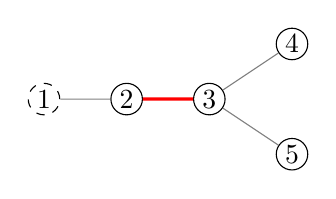
\begin{tikzpicture}[scale=0.7]
			\tikzstyle{Vertex} 	= [circle, draw, solid,  fill=white, minimum size=4mm, inner sep=0pt]
			\tikzstyle{Exposed}	= [dashed]
			\tikzstyle{MC}		= [very thick, red]
			\tikzstyle{NM}		= [gray]
				
			\node (v1) at (0.0, 5) [Vertex][Exposed] {$1$};
			\node (v2) at (1.5, 5) [Vertex] {$2$};
			\node (v3) at (3.0, 5) [Vertex] {$3$};
			\node (v4) at (4.5, 6) [Vertex] {$4$};
			\node (v5) at (4.5, 4) [Vertex] {$5$};
				
			\draw [-] (v1) to (v2) [NM];	
			\draw [-] (v2) to (v3) [MC];
			\draw [-] (v3) to (v4) [NM];
			\draw [-] (v3) to (v5) [NM];
		\end{tikzpicture}
	\end{center}
	}
}

%---------------------slide--------------------%
\frame
{
	\frametitle{Examples of BFS failure on non-bipartite graphs}
	\begin{itemize}
		\item Initial graph
	\end{itemize}
	{\mode<presentation>{\tiny}
	\begin{center}
	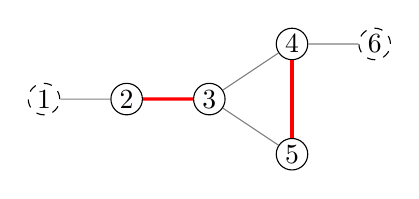
\begin{tikzpicture}[scale=0.7]
		\tikzstyle{Vertex} 	= [circle, draw, solid,  fill=white, minimum size=4mm, inner sep=0pt]
		\tikzstyle{Exposed}	= [dashed]
		\tikzstyle{MC}		= [very thick, red]
		\tikzstyle{NM}		= [gray]
			
		\node (v1) at (0.0, 5) [Vertex][Exposed] {$1$};
		\node (v2) at (1.5, 5) [Vertex] {$2$};
		\node (v3) at (3.0, 5) [Vertex] {$3$};
		\node (v4) at (4.5, 6) [Vertex] {$4$};
		\node (v5) at (4.5, 4) [Vertex] {$5$};
		\node (v6) at (6.0, 6) [Vertex][Exposed] {$6$};
			
		\draw [-] (v1) to (v2) [NM];	
		\draw [-] (v2) to (v3) [MC];
		\draw [-] (v3) to (v4) [NM];
		\draw [-] (v3) to (v5) [NM];
		\draw [-] (v4) to (v5) [MC];
		\draw [-] (v4) to (v6) [NM];	
	\end{tikzpicture}
	\end{center}
	}

	\begin{itemize}
		\item Allow a vertex to be visited at both odd and even levels, we find an augmenting path
	\end{itemize}
	{\mode<presentation>{\tiny}
	\begin{center}
		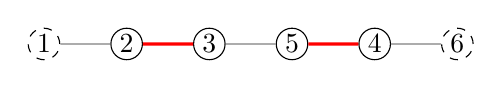
\begin{tikzpicture}[scale=0.7]
			\tikzstyle{Vertex} 	= [circle, draw, solid,  fill=white, minimum size=4mm, inner sep=0pt]
			\tikzstyle{Exposed}	= [dashed]
			\tikzstyle{MC}		= [very thick, red]
			\tikzstyle{NM}		= [gray]
				
			\node (v1) at (0.0, 5) [Vertex][Exposed] {$1$};
			\node (v2) at (1.5, 5) [Vertex] {$2$};
			\node (v3) at (3.0, 5) [Vertex] {$3$};
			\node (v4) at (6.0, 5) [Vertex] {$4$};
			\node (v5) at (4.5, 5) [Vertex] {$5$};
			\node (v6) at (7.5, 5) [Vertex][Exposed] {$6$};
				
			\draw [-] (v1) to (v2) [NM];	
			\draw [-] (v2) to (v3) [MC];
			\draw [-] (v3) to (v5) [NM];
			\draw [-] (v5) to (v4) [MC];
			\draw [-] (v4) to (v6) [NM];
		\end{tikzpicture}
	\end{center}
	}
}

%---------------------slide--------------------%
\frame
{
	\frametitle{Examples of BFS failure on non-bipartite graphs}
	\begin{itemize}
		\item Initial graph
	\end{itemize}
	{\mode<presentation>{\tiny}
	\begin{center}
	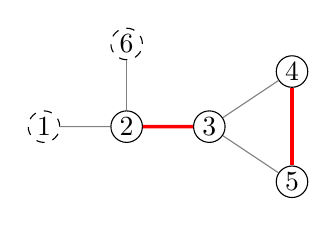
\begin{tikzpicture}[scale=0.7]
		\tikzstyle{Vertex} 	= [circle, draw, solid,  fill=white, minimum size=4mm, inner sep=0pt]
		\tikzstyle{Exposed}	= [dashed]
		\tikzstyle{MC}		= [very thick, red]
		\tikzstyle{NM}		= [gray]
			
		\node (v1) at (0.0, 5) [Vertex][Exposed] {$1$};
		\node (v2) at (1.5, 5) [Vertex] {$2$};
		\node (v3) at (3.0, 5) [Vertex] {$3$};
		\node (v4) at (4.5, 6) [Vertex] {$4$};
		\node (v5) at (4.5, 4) [Vertex] {$5$};
		\node (v6) at (1.5, 6.5) [Vertex][Exposed] {$6$};
			
		\draw [-] (v1) to (v2) [NM];	
		\draw [-] (v2) to (v3) [MC];
		\draw [-] (v3) to (v4) [NM];
		\draw [-] (v3) to (v5) [NM];
		\draw [-] (v4) to (v5) [MC];
		\draw [-] (v2) to (v6) [NM];	
	\end{tikzpicture}
	\end{center}
	}

	\begin{itemize}
		\item But the augmenting path we find may not be a simple path
	\end{itemize}
	{\mode<presentation>{\tiny}
	\begin{center}
		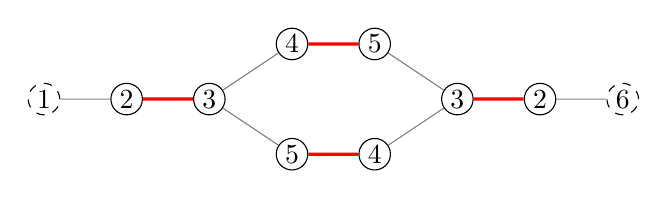
\begin{tikzpicture}[scale=0.7]
			\tikzstyle{Vertex} 	= [circle, draw, solid,  fill=white, minimum size=4mm, inner sep=0pt]
			\tikzstyle{Exposed}	= [dashed]
			\tikzstyle{MC}		= [very thick, red]
			\tikzstyle{NM}		= [gray]
				
			\node (v1) at (0.0, 5) [Vertex][Exposed] {$1$};
			\node (v2) at (1.5, 5) [Vertex] {$2$};
			\node (v22) at (9.0, 5) [Vertex] {$2$};
			\node (v3) at (3.0, 5) [Vertex] {$3$};
			\node (v32) at (7.5, 5) [Vertex] {$3$};
			\node (v4) at (4.5, 6) [Vertex] {$4$};
			\node (v42) at (6.0, 4) [Vertex] {$4$};
			\node (v5) at (6.0, 6) [Vertex] {$5$};
			\node (v52) at (4.5, 4) [Vertex] {$5$};
			\node (v6) at (10.5, 5) [Vertex][Exposed] {$6$};
				
			\draw [-] (v1) to (v2) [NM];	
			\draw [-] (v2) to (v3) [MC];
			\draw [-] (v3) to (v4) [NM];
			\draw [-] (v4) to (v5) [MC];
			\draw [-] (v5) to (v32) [NM];
			\draw [-] (v32) to (v22) [MC];
			\draw [-] (v22) to (v6) [NM];
			\draw [-] (v3) to (v52) [NM];
			\draw [-] (v52) to (v42) [MC];
			\draw [-] (v42) to (v32) [NM];
		\end{tikzpicture}
	\end{center}
	}
}

%---------------------slide--------------------%
\section{Edmonds maximum matching algorithm}
\frame
{
	\frametitle{Alternating Tree}
	\begin{description}
		\item[Alternating Tree] is a tree $J$, each of whose edges joins an odd vertex to an even vertex so that each odd vertex of $J$ meets exactly two edges of $J$.
		\item[-] An alternating tree contains one more even vertex than odd vertices.
	\end{description}
	\begin{center}
	\begin{figure}[h]
	\hfill
		\centering
		\begin{minipage}[c]{.70\textwidth}
			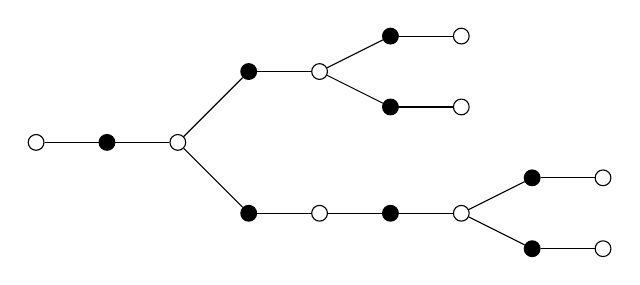
\begin{tikzpicture}[scale=.9]
				\tikzstyle{Flower}	= [circle, fill=white, minimum size=4mm, inner sep=0pt]
				\tikzstyle{Vertex} 	= [circle, draw, solid,  fill=white, minimum size=2mm, inner sep=0pt]
				\tikzstyle{OUT}		= [fill = white]
				\tikzstyle{IN}		= [fill = black]
				\tikzstyle{Exposed}	= [dashed, OUT]
				\tikzstyle{MC}		= [very thick, black]
				\tikzstyle{NM}		= [gray]
				
				\node (v0) at (0,0) [Vertex][OUT] {}; 
				\node (v1) at (1,0) [Vertex][IN] {};
				\node (v2) at (2,0) [Vertex][OUT] {};
				\node (v3) at (3,1) [Vertex][IN] {};
				\node (v4) at (4,1) [Vertex][OUT] {};
				\node (v5) at (5,1.5) [Vertex][IN] {};
				\node (v6) at (6,1.5) [Vertex][OUT] {};
				\node (v7) at (5,0.5) [Vertex][IN] {};
				\node (v8) at (6,0.5) [Vertex][OUT] {};
				\node (v9) at (3,-1) [Vertex][IN] {};
				\node (v10) at(4, -1) [Vertex][OUT] {};
				\node (v11) at(5, -1) [Vertex][IN] {};
				\node (v12) at(6, -1) [Vertex][OUT] {};
				\node (v13) at(7, -0.5) [Vertex][IN] {};
				\node (v14) at(8, -0.5) [Vertex][OUT] {};
				\node (v15) at(7, -1.5) [Vertex][IN] {};
				\node (v16) at(8, -1.5) [Vertex][OUT] {};
				
				\draw [-] (v0) to (v1);
				\draw [-] (v1) to (v2);
				\draw [-] (v2) to (v3);
				\draw [-] (v3) to (v4);
				\draw [-] (v4) to (v5);
				\draw [-] (v5) to (v6);
				\draw [-] (v4) to (v7);
				\draw [-] (v7) to (v8);
				\draw [-] (v2) to (v9);
				\draw [-] (v9) to (v10);
				\draw [-] (v10) to (v11);
				\draw [-] (v11) to (v12);
				\draw [-] (v12) to (v13);
				\draw [-] (v13) to (v14);
				\draw [-] (v12) to (v15);
				\draw [-] (v15) to (v16);	
			\end{tikzpicture}
		\end{minipage}
	\hfill
		\centering
		\begin{minipage}[c]{.20\textwidth}
			\framebox{
			
\begin{tikzpicture}
				\tikzstyle{Flower}	= [circle, fill=white, minimum size=4mm, inner sep=0pt]
				\tikzstyle{Vertex} 	= [circle, draw, solid,  fill=white, minimum size=2mm, inner sep=0pt]
				\tikzstyle{OUT}		= [fill = white]
				\tikzstyle{IN}		= [fill = black]
				\tikzstyle{Exposed}	= [dashed, OUT]
				\tikzstyle{MC}		= [very thick, black]
				\tikzstyle{NM}		= [gray]
				
				\node (v0) at (0,0) [Vertex][OUT][label=right:even vertex] {}; 
				\node (v1) at (0,1) [Vertex][IN][label=right:odd vertex] {};

			\end{tikzpicture}
			}
		\end{minipage}
	\hfill
	\end{figure}
	\end{center}
}

%---------------------slide--------------------%
\frame
{
	\frametitle{Planted Tree}
	\begin{description}
		\item[Planted tree] is an alternating tree $J(M)$ of $G$ for matching $M$ s.t. $M \cap J$ is a maximum matching of $J$.
		\item[Root] is a vertex $r$ in $J$ which is exposed.
	\end{description}

	\begin{center}
		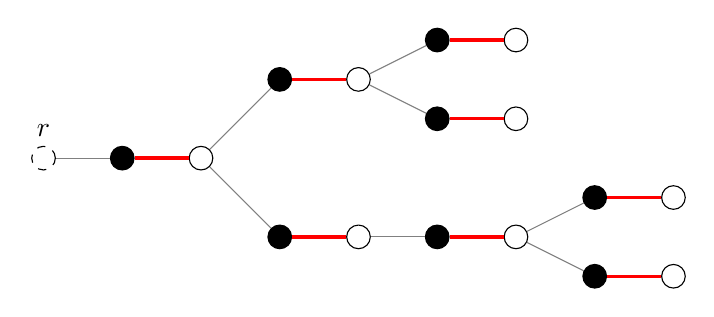
\begin{tikzpicture}
			\tikzstyle{Flower}	= [circle, fill=white, minimum size=4mm, inner sep=0pt]
			\tikzstyle{Vertex} 	= [circle, draw, solid,  fill=white, minimum size=3mm, inner sep=0pt]
			\tikzstyle{OUT}		= [fill = white]
			\tikzstyle{IN}		= [fill = black]
			\tikzstyle{Exposed}	= [dashed, OUT]
			\tikzstyle{MC}		= [very thick, red]
			\tikzstyle{NM}		= [gray]
			
			\node (v0) at (0,0) [Vertex][OUT][Exposed][label=above:$r$] {}; 
			\node (v1) at (1,0) [Vertex][IN] {};
			\node (v2) at (2,0) [Vertex][OUT] {};
			\node (v3) at (3,1) [Vertex][IN] {};
			\node (v4) at (4,1) [Vertex][OUT] {};
			\node (v5) at (5,1.5) [Vertex][IN] {};
			\node (v6) at (6,1.5) [Vertex][OUT] {};
			\node (v7) at (5,0.5) [Vertex][IN] {};
			\node (v8) at (6,0.5) [Vertex][OUT] {};
			\node (v9) at (3,-1) [Vertex][IN] {};
			\node (v10) at(4, -1) [Vertex][OUT] {};
			\node (v11) at(5, -1) [Vertex][IN] {};
			\node (v12) at(6, -1) [Vertex][OUT] {};
			\node (v13) at(7, -0.5) [Vertex][IN] {};
			\node (v14) at(8, -0.5) [Vertex][OUT] {};
			\node (v15) at(7, -1.5) [Vertex][IN] {};
			\node (v16) at(8, -1.5) [Vertex][OUT] {};
			
			\draw [-] (v0) to (v1) [NM];
			\draw [-] (v1) to (v2) [MC];
			\draw [-] (v2) to (v3) [NM];
			\draw [-] (v3) to (v4) [MC];
			\draw [-] (v4) to (v5) [NM];
			\draw [-] (v5) to (v6) [MC];
			\draw [-] (v4) to (v7) [NM];
			\draw [-] (v7) to (v8) [MC];
			\draw [-] (v2) to (v9) [NM];
			\draw [-] (v9) to (v10) [MC];
			\draw [-] (v10) to (v11) [NM];
			\draw [-] (v11) to (v12) [MC];
			\draw [-] (v12) to (v13) [NM];
			\draw [-] (v13) to (v14) [MC];
			\draw [-] (v12) to (v15) [NM];
			\draw [-] (v15) to (v16) [MC];	
		\end{tikzpicture}
	\end{center}
}

%---------------------slide--------------------%
\frame
{
	\frametitle{Planted Tree}
	\begin{beamercolorbox}[sep=1em,wd=11cm]{postit}
		In planted tree $J(M)$ every alternating path $P(M)$, which has even vertex $v$ and the matching edge to $v$ at one of its ends, is a subpath of the alternating path $P_{v}(M)$ in $J(M)$ which joins $v$ to the root $r$.
	\end{beamercolorbox}

	\begin{center}
		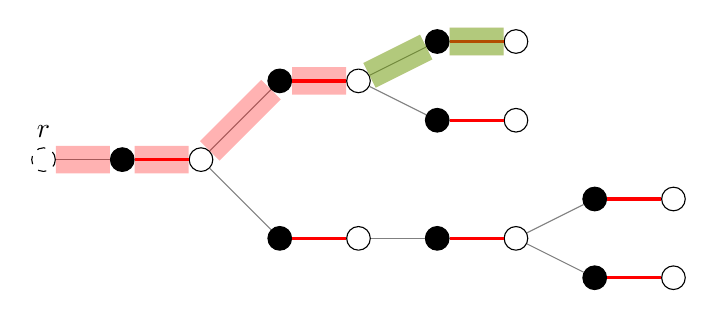
\begin{tikzpicture}
			\tikzstyle{Flower}	= [circle, fill=white, minimum size=4mm, inner sep=0pt]
			\tikzstyle{Vertex} 	= [circle, draw, solid,  fill=white, minimum size=3mm, inner sep=0pt]
			\tikzstyle{OUT}		= [fill = white]
			\tikzstyle{IN}		= [fill = black]
			\tikzstyle{Exposed}	= [dashed, OUT]
			\tikzstyle{MC}		= [very thick, red]
			\tikzstyle{NM}		= [gray]
			
			\node (v0) at (0,0) [Vertex][OUT][Exposed][label=above:$r$] {}; 
			\node (v1) at (1,0) [Vertex][IN] {};
			\node (v2) at (2,0) [Vertex][OUT] {};
			\node (v3) at (3,1) [Vertex][IN] {};
			\node (v4) at (4,1) [Vertex][OUT] {};
			\node (v5) at (5,1.5) [Vertex][IN] {};
			\node (v6) at (6,1.5) [Vertex][OUT] {};
			\node (v7) at (5,0.5) [Vertex][IN] {};
			\node (v8) at (6,0.5) [Vertex][OUT] {};
			\node (v9) at (3,-1) [Vertex][IN] {};
			\node (v10) at(4, -1) [Vertex][OUT] {};
			\node (v11) at(5, -1) [Vertex][IN] {};
			\node (v12) at(6, -1) [Vertex][OUT] {};
			\node (v13) at(7, -0.5) [Vertex][IN] {};
			\node (v14) at(8, -0.5) [Vertex][OUT] {};
			\node (v15) at(7, -1.5) [Vertex][IN] {};
			\node (v16) at(8, -1.5) [Vertex][OUT] {};
			
			\draw [-] (v0) to (v1) [NM];
			\draw [-] (v1) to (v2) [MC];
			\draw [-] (v2) to (v3) [NM];
			\draw [-] (v3) to (v4) [MC];
			\draw [-] (v4) to (v5) [NM];
			\draw [-] (v5) to (v6) [MC];
			\draw [-] (v4) to (v7) [NM];
			\draw [-] (v7) to (v8) [MC];
			\draw [-] (v2) to (v9) [NM];
			\draw [-] (v9) to (v10) [MC];
			\draw [-] (v10) to (v11) [NM];
			\draw [-] (v11) to (v12) [MC];
			\draw [-] (v12) to (v13) [NM];
			\draw [-] (v13) to (v14) [MC];
			\draw [-] (v12) to (v15) [NM];
			\draw [-] (v15) to (v16) [MC];
			
			\draw (v0) -- (v1) -- (v2) -- (v3) -- (v4) -- (v5) -- (v6) [line width=10pt, red, opacity=0.3];
			\draw (v4) -- (v5) -- (v6) [line width=10pt, green, opacity=0.3];
		\end{tikzpicture}
	\end{center}
	
	From any vertex in the planted tree we can easily find the path back to the root!
}

%---------------------slide--------------------%
\frame
{
	\frametitle{Augmenting Tree}
	\begin{description}
		\item[Augmenting tree] is a planted tree $J(M)$ plus an edge $e$ of $G$ such that one end-point of $e$ is an even vertex $v_{1}$ of $J$ and the other end-point $v_{2}$ is exposed not in $J$.
	\end{description}

	\begin{center}
		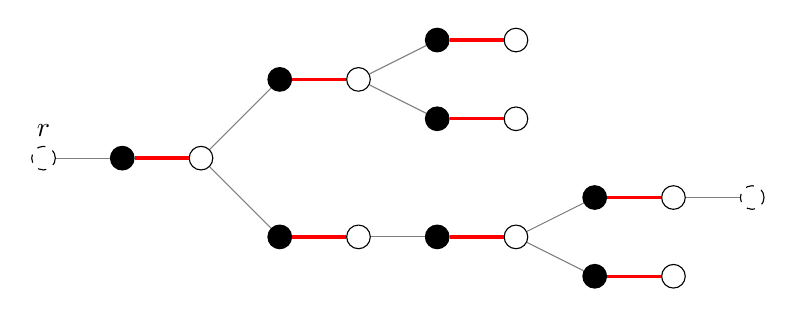
\begin{tikzpicture}
			\tikzstyle{Flower}	= [circle, fill=white, minimum size=4mm, inner sep=0pt]
			\tikzstyle{Vertex} 	= [circle, draw, solid,  fill=white, minimum size=3mm, inner sep=0pt]
			\tikzstyle{OUT}		= [fill = white]
			\tikzstyle{IN}		= [fill = black]
			\tikzstyle{Exposed}	= [dashed, OUT]
			\tikzstyle{MC}		= [very thick, red]
			\tikzstyle{NM}		= [gray]
			
			\node (v0) at (0,0) [Vertex][OUT][Exposed][label=above:$r$] {}; 
			\node (v1) at (1,0) [Vertex][IN] {};
			\node (v2) at (2,0) [Vertex][OUT] {};
			\node (v3) at (3,1) [Vertex][IN] {};
			\node (v4) at (4,1) [Vertex][OUT] {};
			\node (v5) at (5,1.5) [Vertex][IN] {};
			\node (v6) at (6,1.5) [Vertex][OUT] {};
			\node (v7) at (5,0.5) [Vertex][IN] {};
			\node (v8) at (6,0.5) [Vertex][OUT] {};
			\node (v9) at (3,-1) [Vertex][IN] {};
			\node (v10) at(4, -1) [Vertex][OUT] {};
			\node (v11) at(5, -1) [Vertex][IN] {};
			\node (v12) at(6, -1) [Vertex][OUT] {};
			\node (v13) at(7, -0.5) [Vertex][IN] {};
			\node (v14) at(8, -0.5) [Vertex][OUT] {};
			\node (v15) at(7, -1.5) [Vertex][IN] {};
			\node (v16) at(8, -1.5) [Vertex][OUT] {};
			\node (v17) at(9, -0.5) [Vertex][OUT][Exposed] {};
			
			\draw [-] (v0) to (v1) [NM];
			\draw [-] (v1) to (v2) [MC];
			\draw [-] (v2) to (v3) [NM];
			\draw [-] (v3) to (v4) [MC];
			\draw [-] (v4) to (v5) [NM];
			\draw [-] (v5) to (v6) [MC];
			\draw [-] (v4) to (v7) [NM];
			\draw [-] (v7) to (v8) [MC];
			\draw [-] (v2) to (v9) [NM];
			\draw [-] (v9) to (v10) [MC];
			\draw [-] (v10) to (v11) [NM];
			\draw [-] (v11) to (v12) [MC];
			\draw [-] (v12) to (v13) [NM];
			\draw [-] (v13) to (v14) [MC];
			\draw [-] (v12) to (v15) [NM];
			\draw [-] (v15) to (v16) [MC];
			\draw [-] (v14) to (v17) [NM];
		\end{tikzpicture}
	\end{center}
}

%---------------------slide--------------------%
\frame
{
	\frametitle{Stem}
	\begin{description}
		\item[Stem] is an alternating path with an exposed vertex at one end and a matching edge at the other end.
		\item[Tip] is the non-exposed end vertex in the stem.
	\end{description}
	\begin{center}
		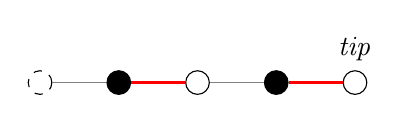
\begin{tikzpicture}
			\tikzstyle{Flower}	= [circle, fill=white, minimum size=4mm, inner sep=0pt]
			\tikzstyle{Vertex} 	= [circle, draw, solid,  fill=white, minimum size=3mm, inner sep=0pt]
			\tikzstyle{OUT}		= [fill = white]
			\tikzstyle{IN}		= [fill = black]
			\tikzstyle{Exposed}	= [dashed, OUT]
			\tikzstyle{MC}		= [very thick, red]
			\tikzstyle{NM}		= [gray]
			
			\node (v0) at (0,1) [Vertex][OUT][Exposed] {}; 
			\node (v1) at (1,1) [Vertex][IN] {};
			\node (v2) at (2,1) [Vertex][OUT] {};
			\node (v3) at (3,1) [Vertex][IN] {};
			\node (v4) at (4,1) [Vertex][OUT][label=above:\emph{tip}] {};
			
			\draw [-] (v0) to (v1) [NM];
			\draw [-] (v1) to (v2) [MC];
			\draw [-] (v2) to (v3) [NM];
			\draw [-] (v3) to (v4) [MC];
		\end{tikzpicture}
	\end{center}
}

%---------------------slide--------------------%
\frame
{
	\frametitle{Blossom}
	\begin{description}
		\item[Blossom] is an odd cycle in $G$ for which $M \cap B$ is a maximum matching in $B$ with one vertex exposed for $M \cap B$.
	\end{description}
	\begin{center}
		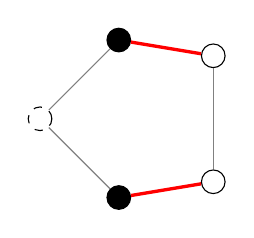
\begin{tikzpicture}
			\tikzstyle{Flower}	= [circle, fill=white, minimum size=4mm, inner sep=0pt]
			\tikzstyle{Vertex} 	= [circle, draw, solid,  fill=white, minimum size=3mm, inner sep=0pt]
			\tikzstyle{OUT}		= [fill = white]
			\tikzstyle{IN}		= [fill = black]
			\tikzstyle{Exposed}	= [dashed, OUT]
			\tikzstyle{MC}		= [very thick, red]
			\tikzstyle{NM}		= [gray]
			
			\node (v4) at (4,1) [Vertex][Exposed][OUT] {};
			\node (v5) at (5,2) [Vertex][IN] {};
			\node (v6) at (6.2, 1.8) [Vertex][OUT] {};
			\node (v7) at (5,0) [Vertex][IN] {};
			\node (v8) at (6.2, 0.2) [Vertex][OUT] {};
			
			\draw [-] (v4) to (v5) [NM];
			\draw [-] (v5) to (v6) [MC];
			\draw [-] (v4) to (v7) [NM];
			\draw [-] (v7) to (v8) [MC];
			\draw [-] (v8) to (v6) [NM];
		\end{tikzpicture}
	\end{center}
}

%---------------------slide--------------------%
\frame
{
	\frametitle{Flower}
	\begin{description}
		\item[Flower] consists of a blossom and a stem which intersect only at the tip of the stem.
	\end{description}
	\begin{center}
		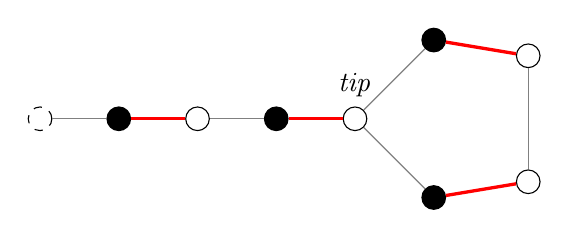
\begin{tikzpicture}
			\tikzstyle{Flower}	= [circle, fill=white, minimum size=4mm, inner sep=0pt]
			\tikzstyle{Vertex} 	= [circle, draw, solid,  fill=white, minimum size=3mm, inner sep=0pt]
			\tikzstyle{OUT}		= [fill = white]
			\tikzstyle{IN}		= [fill = black]
			\tikzstyle{Exposed}	= [dashed, OUT]
			\tikzstyle{MC}		= [very thick, red]
			\tikzstyle{NM}		= [gray]
			
			\node (v0) at (0,1) [Vertex][OUT][Exposed] {}; 
			\node (v1) at (1,1) [Vertex][IN] {};
			\node (v2) at (2,1) [Vertex][OUT] {};
			\node (v3) at (3,1) [Vertex][IN] {};
			\node (v4) at (4,1) [Vertex][OUT][label=above:\emph{tip}] {};
			\node (v5) at (5,2) [Vertex][IN] {};
			\node (v6) at (6.2, 1.8) [Vertex][OUT] {};
			\node (v7) at (5,0) [Vertex][IN] {};
			\node (v8) at (6.2, 0.2) [Vertex][OUT] {};
			
			\draw [-] (v0) to (v1) [NM];
			\draw [-] (v1) to (v2) [MC];
			\draw [-] (v2) to (v3) [NM];
			\draw [-] (v3) to (v4) [MC];
			\draw [-] (v4) to (v5) [NM];
			\draw [-] (v5) to (v6) [MC];
			\draw [-] (v4) to (v7) [NM];
			\draw [-] (v7) to (v8) [MC];
			\draw [-] (v8) to (v6) [NM];
		\end{tikzpicture}
	\end{center}
}

%---------------------slide--------------------%
\frame
{
	\frametitle{Flowered tree}
	\begin{description}
		\item[Flowered tree] is a planted tree $J$ plus an edge $e$ of $G$ which joins a pair of even vertices of $J$. The union of $e$ and the two paths which join its even-vertex end-points to the root of of $J$ is a flower, $F$.
	\end{description}

	\begin{center}
		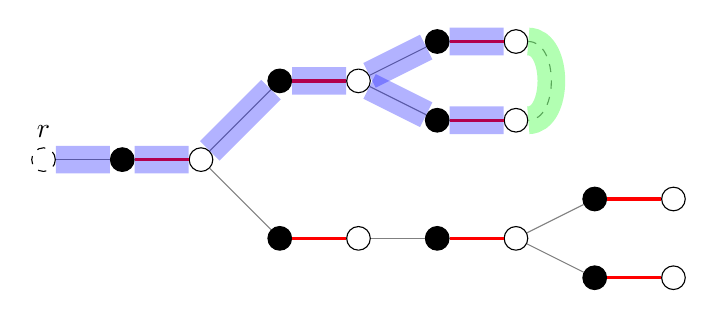
\begin{tikzpicture}
			\tikzstyle{Flower}	= [circle, fill=white, minimum size=4mm, inner sep=0pt]
			\tikzstyle{Vertex} 	= [circle, draw, solid,  fill=white, minimum size=3mm, inner sep=0pt]
			\tikzstyle{OUT}		= [fill = white]
			\tikzstyle{IN}		= [fill = black]
			\tikzstyle{Exposed}	= [dashed, OUT]
			\tikzstyle{MC}		= [very thick, red]
			\tikzstyle{NM}		= [gray]
			\tikzstyle{DS}		= [gray, dashed]
			
			\node (v0) at (0,0) [Vertex][OUT][Exposed][label=above:$r$] {}; 
			\node (v1) at (1,0) [Vertex][IN] {};
			\node (v2) at (2,0) [Vertex][OUT] {};
			\node (v3) at (3,1) [Vertex][IN] {};
			\node (v4) at (4,1) [Vertex][OUT] {};
			\node (v5) at (5,1.5) [Vertex][IN] {};
			\node (v6) at (6,1.5) [Vertex][OUT] {};
			\node (v7) at (5,0.5) [Vertex][IN] {};
			\node (v8) at (6,0.5) [Vertex][OUT] {};
			\node (v9) at (3,-1) [Vertex][IN] {};
			\node (v10) at(4, -1) [Vertex][OUT] {};
			\node (v11) at(5, -1) [Vertex][IN] {};
			\node (v12) at(6, -1) [Vertex][OUT] {};
			\node (v13) at(7, -0.5) [Vertex][IN] {};
			\node (v14) at(8, -0.5) [Vertex][OUT] {};
			\node (v15) at(7, -1.5) [Vertex][IN] {};
			\node (v16) at(8, -1.5) [Vertex][OUT] {};
			
			\draw [-] (v0) to (v1) [NM];
			\draw [-] (v1) to (v2) [MC];
			\draw [-] (v2) to (v3) [NM];
			\draw [-] (v3) to (v4) [MC];
			\draw [-] (v4) to (v5) [NM];
			\draw [-] (v5) to (v6) [MC];
			\draw [-] (v4) to (v7) [NM];
			\draw [-] (v7) to (v8) [MC];
			\draw [-] (v2) to (v9) [NM];
			\draw [-] (v9) to (v10) [MC];
			\draw [-] (v10) to (v11) [NM];
			\draw [-] (v11) to (v12) [MC];
			\draw [-] (v12) to (v13) [NM];
			\draw [-] (v13) to (v14) [MC];
			\draw [-] (v12) to (v15) [NM];
			\draw [-] (v15) to (v16) [MC];
			\draw [-] (v6) to [in=0, out=0](v8) [DS];
			\draw (v0) -- (v1) -- (v2) -- (v3) -- (v4) -- (v5) -- (v6) [line width=10pt, blue, opacity=0.3];
			\draw (v4) -- (v7) -- (v8) [line width=10pt, blue, opacity=0.3];
			\draw [-] (v6) to [in=0, out=0](v8) [line width=10pt, green, opacity=0.3];
		\end{tikzpicture}
	\end{center}
}

%---------------------slide--------------------%
\frame
{
	\frametitle{Hungarian tree}
	\begin{description}
		\item[Hungarian tree] is an alternating tree whose even vertices are joined by edges of $G$ only to its inner vertices.
	\end{description}

	\begin{center}
		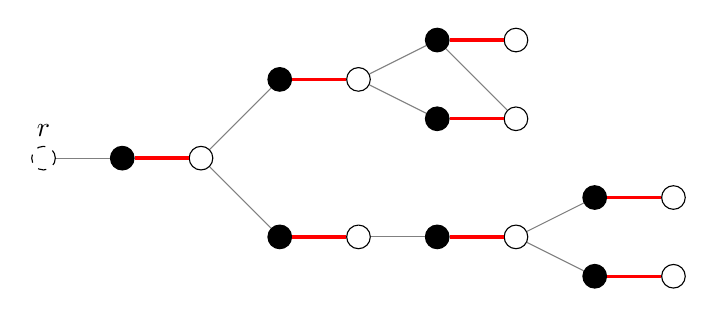
\begin{tikzpicture}
			\tikzstyle{Flower}	= [circle, fill=white, minimum size=4mm, inner sep=0pt]
			\tikzstyle{Vertex} 	= [circle, draw, solid,  fill=white, minimum size=3mm, inner sep=0pt]
			\tikzstyle{OUT}		= [fill = white]
			\tikzstyle{IN}		= [fill = black]
			\tikzstyle{Exposed}	= [dashed, OUT]
			\tikzstyle{MC}		= [very thick, red]
			\tikzstyle{NM}		= [gray]
			\tikzstyle{DS}		= [gray, dashed]
			
			\node (v0) at (0,0) [Vertex][OUT][Exposed][label=above:$r$] {}; 
			\node (v1) at (1,0) [Vertex][IN] {};
			\node (v2) at (2,0) [Vertex][OUT] {};
			\node (v3) at (3,1) [Vertex][IN] {};
			\node (v4) at (4,1) [Vertex][OUT] {};
			\node (v5) at (5,1.5) [Vertex][IN] {};
			\node (v6) at (6,1.5) [Vertex][OUT] {};
			\node (v7) at (5,0.5) [Vertex][IN] {};
			\node (v8) at (6,0.5) [Vertex][OUT] {};
			\node (v9) at (3,-1) [Vertex][IN] {};
			\node (v10) at(4, -1) [Vertex][OUT] {};
			\node (v11) at(5, -1) [Vertex][IN] {};
			\node (v12) at(6, -1) [Vertex][OUT] {};
			\node (v13) at(7, -0.5) [Vertex][IN] {};
			\node (v14) at(8, -0.5) [Vertex][OUT] {};
			\node (v15) at(7, -1.5) [Vertex][IN] {};
			\node (v16) at(8, -1.5) [Vertex][OUT] {};
			
			\draw [-] (v0) to (v1) [NM];
			\draw [-] (v1) to (v2) [MC];
			\draw [-] (v2) to (v3) [NM];
			\draw [-] (v3) to (v4) [MC];
			\draw [-] (v4) to (v5) [NM];
			\draw [-] (v5) to (v6) [MC];
			\draw [-] (v4) to (v7) [NM];
			\draw [-] (v7) to (v8) [MC];
			\draw [-] (v2) to (v9) [NM];
			\draw [-] (v9) to (v10) [MC];
			\draw [-] (v10) to (v11) [NM];
			\draw [-] (v11) to (v12) [MC];
			\draw [-] (v12) to (v13) [NM];
			\draw [-] (v13) to (v14) [MC];
			\draw [-] (v12) to (v15) [NM];
			\draw [-] (v15) to (v16) [MC];
			\draw [-] (v5) to (v8) [NM];
		\end{tikzpicture}
	\end{center}
}

%---------------------slide--------------------%
\frame
{
	\frametitle{Shrinking the blossom}
	\uncover<1->{
	\begin{center}
		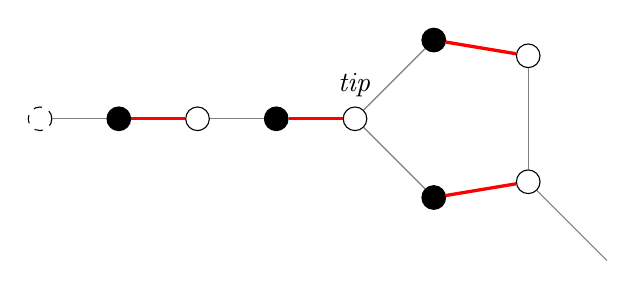
\begin{tikzpicture}
			\tikzstyle{Flower}	= [circle, fill=white, minimum size=4mm, inner sep=0pt]
			\tikzstyle{Vertex} 	= [circle, draw, solid,  fill=white, minimum size=3mm, inner sep=0pt]
			\tikzstyle{OUT}		= [fill = white]
			\tikzstyle{IN}		= [fill = black]
			\tikzstyle{Exposed}	= [dashed, OUT]
			\tikzstyle{MC}		= [very thick, red]
			\tikzstyle{NM}		= [gray]
			
			\node (v0) at (0,1) [Vertex][OUT][Exposed] {}; 
			\node (v1) at (1,1) [Vertex][IN] {};
			\node (v2) at (2,1) [Vertex][OUT] {};
			\node (v3) at (3,1) [Vertex][IN] {};
			\node (v4) at (4,1) [Vertex][OUT][label=above:\emph{tip}] {};
			\node (v5) at (5,2) [Vertex][IN] {};
			\node (v6) at (6.2, 1.8) [Vertex][OUT] {};
			\node (v7) at (5,0) [Vertex][IN] {};
			\node (v8) at (6.2, 0.2) [Vertex][OUT] {};
			
			\draw [-] (v0) to (v1) [NM];
			\draw [-] (v1) to (v2) [MC];
			\draw [-] (v2) to (v3) [NM];
			\draw [-] (v3) to (v4) [MC];
			\draw [-] (v4) to (v5) [NM];
			\draw [-] (v5) to (v6) [MC];
			\draw [-] (v4) to (v7) [NM];
			\draw [-] (v7) to (v8) [MC];
			\draw [-] (v8) to (v6) [NM];

			%\draw [-] (v6) to (7.2, 2.8) [NM];
			\draw [-] (v8) to (7.2, -.8) [NM];
		\end{tikzpicture}
	\end{center}}
	
	\uncover<2->{
	\begin{center}
		
\begin{tikzpicture}			
			\draw [->] (0,1) to (0,0) [very thick] node [right, midway] {shirnk};
		\end{tikzpicture}
	\end{center}

	\begin{center}
		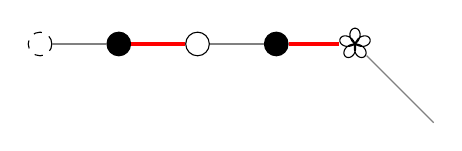
\begin{tikzpicture}
			\tikzstyle{Flower}	= [circle, fill=white, minimum size=4mm, inner sep=0pt]
			\tikzstyle{Vertex} 	= [circle, draw, solid,  fill=white, minimum size=3mm, inner sep=0pt]
			\tikzstyle{OUT}		= [fill = white]
			\tikzstyle{IN}		= [fill = black]
			\tikzstyle{Exposed}	= [dashed, OUT]
			\tikzstyle{MC}		= [very thick, red]
			\tikzstyle{NM}		= [gray]
			
			\node (v0) at (0,1) [Vertex][OUT][Exposed] {}; 
			\node (v1) at (1,1) [Vertex][IN] {};
			\node (v2) at (2,1) [Vertex][OUT] {};
			\node (v3) at (3,1) [Vertex][IN] {};
			\node (v4) at (4,1) [Flower][OUT] {};
			\pgfplothandlerlineto
			\pgfplotfunction{\x}{0, 3, ..., 540}{
				\pgfpointxy     
				{-0.2 * cos(\x) * sin(5 / 3 * \x) + 4}
				{-0.2 * sin(\x) * sin(5 / 3 * \x) + 1}
			}
			\pgfusepath{stroke}
			
			\draw [-] (v0) to (v1) [NM];
			\draw [-] (v1) to (v2) [MC];
			\draw [-] (v2) to (v3) [NM];
			\draw [-] (v3) to (v4) [MC];

			%\draw [-] (v4) to (5, 2) [NM];
			\draw [-] (v4) to (5, 0) [NM];
		\end{tikzpicture}
	\end{center}}
}

%---------------------slide--------------------%
\frame
{
	\frametitle{Correctness of the algorithm}
	\begin{block}{Theorem}
		$M$ is a maximum size matching in $G$ if and only if $M/B$ is maximum size matching in $G/B$.
	\end{block}
	\begin{center}
		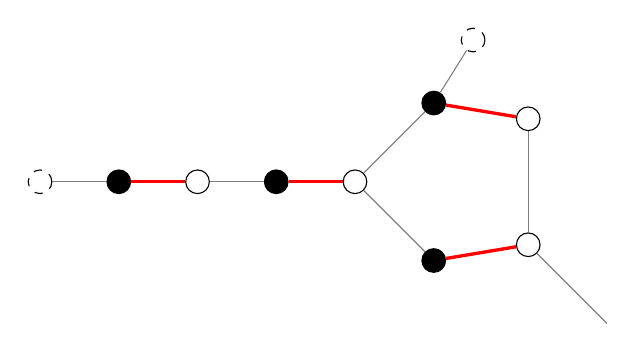
\begin{tikzpicture}
			\tikzstyle{Flower}	= [circle, fill=white, minimum size=4mm, inner sep=0pt]
			\tikzstyle{Vertex} 	= [circle, draw, solid,  fill=white, minimum size=3mm, inner sep=0pt]
			\tikzstyle{OUT}		= [fill = white]
			\tikzstyle{IN}		= [fill = black]
			\tikzstyle{Exposed}	= [dashed, OUT]
			\tikzstyle{MC}		= [very thick, red]
			\tikzstyle{NM}		= [gray]
			
			\node (v0) at (0,1) [Vertex][OUT][Exposed] {}; 
			\node (v1) at (1,1) [Vertex][IN] {};
			\node (v2) at (2,1) [Vertex][OUT] {};
			\node (v3) at (3,1) [Vertex][IN] {};
			\node (v4) at (4,1) [Vertex][OUT] {};
			\node (v5) at (5,2) [Vertex][IN] {};
			\node (v6) at (6.2, 1.8) [Vertex][OUT] {};
			\node (v7) at (5,0) [Vertex][IN] {};
			\node (v8) at (6.2, 0.2) [Vertex][OUT] {};

			\node (v9) at (5.5, 2.8) [Vertex][OUT][Exposed] {};
			
			\draw [-] (v0) to (v1) [NM];
			\draw [-] (v1) to (v2) [MC];
			\draw [-] (v2) to (v3) [NM];
			\draw [-] (v3) to (v4) [MC];
			\draw [-] (v4) to (v5) [NM];
			\draw [-] (v5) to (v6) [MC];
			\draw [-] (v4) to (v7) [NM];
			\draw [-] (v7) to (v8) [MC];
			\draw [-] (v8) to (v6) [NM];

			\draw [-] (v5) to (v9) [NM];
			\draw [-] (v8) to (7.2, -.8) [NM];
		\end{tikzpicture}
	\end{center}
}

%---------------------slide--------------------%
\frame
{
	\frametitle{Correctness of the algorithm}
	\begin{block}{Theorem}
		$M$ is a maximum size matching in $G$ if and only if $M/B$ is maximum size matching in $G/B$.
	\end{block}
	\begin{center}
		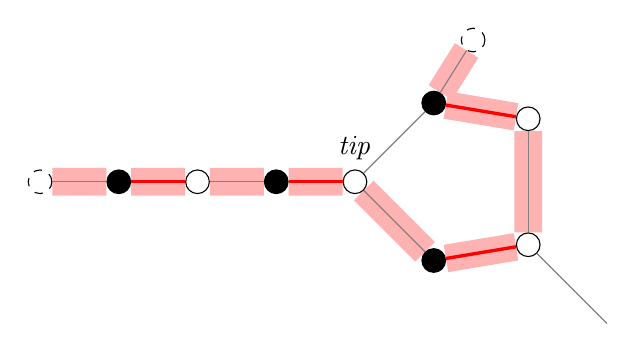
\begin{tikzpicture}
			\tikzstyle{Flower}	= [circle, fill=white, minimum size=4mm, inner sep=0pt]
			\tikzstyle{Vertex} 	= [circle, draw, solid,  fill=white, minimum size=3mm, inner sep=0pt]
			\tikzstyle{OUT}		= [fill = white]
			\tikzstyle{IN}		= [fill = black]
			\tikzstyle{Exposed}	= [dashed, OUT]
			\tikzstyle{MC}		= [very thick, red]
			\tikzstyle{NM}		= [gray]
			
			\node (v0) at (0,1) [Vertex][OUT][Exposed] {}; 
			\node (v1) at (1,1) [Vertex][IN] {};
			\node (v2) at (2,1) [Vertex][OUT] {};
			\node (v3) at (3,1) [Vertex][IN] {};
			\node (v4) at (4,1) [Vertex][OUT][label=above:\emph{tip}] {};
			\node (v5) at (5,2) [Vertex][IN] {};
			\node (v6) at (6.2, 1.8) [Vertex][OUT] {};
			\node (v7) at (5,0) [Vertex][IN] {};
			\node (v8) at (6.2, 0.2) [Vertex][OUT] {};

			\node (v9) at (5.5, 2.8) [Vertex][OUT][Exposed] {};

			\draw (v0) -- (v1) -- (v2) -- (v3) -- (v4) -- (v7) -- (v8) -- (v6) -- (v5) --  (v9) [line width=10pt, red, opacity=0.3];
			
			\draw [-] (v0) to (v1) [NM];
			\draw [-] (v1) to (v2) [MC];
			\draw [-] (v2) to (v3) [NM];
			\draw [-] (v3) to (v4) [MC];
			\draw [-] (v4) to (v5) [NM];
			\draw [-] (v5) to (v6) [MC];
			\draw [-] (v4) to (v7) [NM];
			\draw [-] (v7) to (v8) [MC];
			\draw [-] (v8) to (v6) [NM];

			\draw [-] (v5) to (v9) [NM];
			\draw [-] (v8) to (7.2, -.8) [NM];
		\end{tikzpicture}
	\end{center}
	
	\begin{center}
		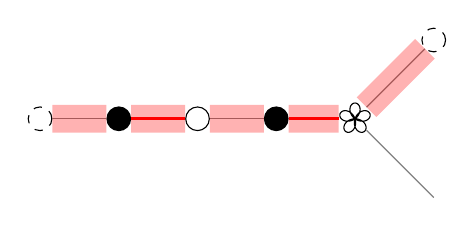
\begin{tikzpicture}
			\tikzstyle{Flower}	= [circle, fill=white, minimum size=4mm, inner sep=0pt]
			\tikzstyle{Vertex} 	= [circle, draw, solid,  fill=white, minimum size=3mm, inner sep=0pt]
			\tikzstyle{OUT}		= [fill = white]
			\tikzstyle{IN}		= [fill = black]
			\tikzstyle{Exposed}	= [dashed, OUT]
			\tikzstyle{MC}		= [very thick, red]
			\tikzstyle{NM}		= [gray]
			
			\node (v0) at (0,1) [Vertex][OUT][Exposed] {}; 
			\node (v1) at (1,1) [Vertex][IN] {};
			\node (v2) at (2,1) [Vertex][OUT] {};
			\node (v3) at (3,1) [Vertex][IN] {};
			\node (v4) at (4,1) [Flower][OUT] {};
			
			\node (v5) at (5, 2) [Vertex][OUT][Exposed] {};
			
			\pgfplothandlerlineto
			\pgfplotfunction{\x}{0, 3, ..., 540}{
				\pgfpointxy     
				{-0.2 * cos(\x) * sin(5 / 3 * \x) + 4}
				{-0.2 * sin(\x) * sin(5 / 3 * \x) + 1}
			}
			\pgfusepath{stroke}
				
			\draw [-] (v0) to (v1) [NM];
			\draw [-] (v1) to (v2) [MC];
			\draw [-] (v2) to (v3) [NM];
			\draw [-] (v3) to (v4) [MC];
	
			\draw [-] (v4) to (v5) [NM];
			\draw [-] (v4) to (5, 0) [NM];
			
			\draw (v0) -- (v1) -- (v2) -- (v3) -- (v4) -- (v5) [line width=10pt, red, opacity=0.3];
		\end{tikzpicture}
	\end{center}
}

%---------------------slide--------------------%
\frame
{
	\frametitle{Examples}
	{
	A graph $G=(V,E)$ and a matching $M$.
	
	\begin{center}
	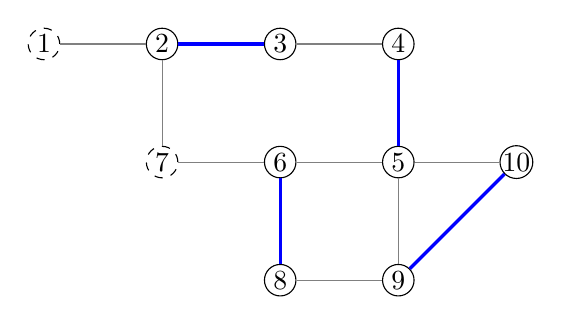
\begin{tikzpicture}
		\tikzstyle{Flower}	= [circle, fill=white, minimum size=4mm, inner sep=0pt]
		\tikzstyle{Vertex} 	= [circle, draw, solid,  fill=white, minimum size=4mm, inner sep=0pt]
		\tikzstyle{OUT}		= [fill = white]
		\tikzstyle{IN}		= [fill = black]
		\tikzstyle{Exposed}	= [dashed, OUT]
		\tikzstyle{MC}		= [very thick, blue]
		\tikzstyle{NM}		= [gray]
		
		\node (v1) at (0.0, 5.0) [Vertex][Exposed] {$1$};
		\node (v2) at (1.5, 5.0) [Vertex] {$2$};
		\node (v3) at (3.0, 5.0) [Vertex] {$3$};
		\node (v4) at (4.5, 5.0) [Vertex] {$4$};
		\node (v5) at (4.5, 3.5) [Vertex] {$5$};
		\node (v6) at (3.0, 3.5) [Vertex] {$6$};
		\node (v7) at (1.5, 3.5) [Vertex][Exposed] {$7$};
		\node (v8) at (3.0, 2.0) [Vertex] {$8$};
		\node (v9) at (4.5, 2.0) [Vertex] {$9$};
		\node (v10) at (6.0, 3.5) [Vertex] {$10$};
		
		\draw [-] (v1) to (v2) [NM];
		\draw [-] (v2) to (v3) [MC];
		\draw [-] (v2) to (v7) [NM];
		\draw [-] (v3) to (v4) [NM];
		\draw [-] (v4) to (v5) [MC];
		\draw [-] (v5) to (v6) [NM];
		\draw [-] (v5) to (v9) [NM];
		\draw [-] (v5) to (v10) [NM];
		\draw [-] (v6) to (v7) [NM];
		\draw [-] (v6) to (v8) [MC];
		\draw [-] (v8) to (v9) [NM];
		\draw [-] (v9) to (v10) [MC];
	\end{tikzpicture}
	\end{center}
	}
}

%---------------------slide--------------------%
\frame
{
	\frametitle{Examples}
	{\scriptsize
	A graph $G=(V,E)$ and a matching $M$.
	
	\begin{center}
	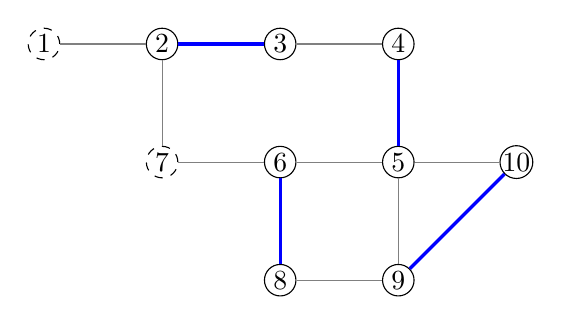
\begin{tikzpicture}
		\tikzstyle{Flower}	= [circle, fill=white, minimum size=4mm, inner sep=0pt]
		\tikzstyle{Vertex} 	= [circle, draw, solid,  fill=white, minimum size=4mm, inner sep=0pt]
		\tikzstyle{OUT}		= [fill = white]
		\tikzstyle{IN}		= [fill = black]
		\tikzstyle{Exposed}	= [dashed, OUT]
		\tikzstyle{MC}		= [very thick, blue]
		\tikzstyle{NM}		= [gray]
		
		\node (v1) at (0.0, 5.0) [Vertex][Exposed] {$1$};
		\node (v2) at (1.5, 5.0) [Vertex] {$2$};
		\node (v3) at (3.0, 5.0) [Vertex] {$3$};
		\node (v4) at (4.5, 5.0) [Vertex] {$4$};
		\node (v5) at (4.5, 3.5) [Vertex] {$5$};
		\node (v6) at (3.0, 3.5) [Vertex] {$6$};
		\node (v7) at (1.5, 3.5) [Vertex][Exposed] {$7$};
		\node (v8) at (3.0, 2.0) [Vertex] {$8$};
		\node (v9) at (4.5, 2.0) [Vertex] {$9$};
		\node (v10) at (6.0, 3.5) [Vertex] {$10$};
		
		\draw [-] (v1) to (v2) [NM];
		\draw [-] (v2) to (v3) [MC];
		\draw [-] (v2) to (v7) [NM];
		\draw [-] (v3) to (v4) [NM];
		\draw [-] (v4) to (v5) [MC];
		\draw [-] (v5) to (v6) [NM];
		\draw [-] (v5) to (v9) [NM];
		\draw [-] (v5) to (v10) [NM];
		\draw [-] (v6) to (v7) [NM];
		\draw [-] (v6) to (v8) [MC];
		\draw [-] (v8) to (v9) [NM];
		\draw [-] (v9) to (v10) [MC];
	\end{tikzpicture}
	\end{center}

	Start a BFS from 1. An exposed vertex is a planted tree.
	
	\begin{center}
	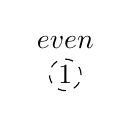
\begin{tikzpicture}
		\tikzstyle{Flower}	= [circle, fill=white, minimum size=4mm, inner sep=0pt]
		\tikzstyle{Vertex} 	= [circle, draw, solid,  fill=white, minimum size=4mm, inner sep=0pt]
		\tikzstyle{OUT}		= [fill = white]
		\tikzstyle{IN}		= [fill = black]
		\tikzstyle{Exposed}	= [dashed, OUT]
		\tikzstyle{MC}		= [very thick, blue]
		\tikzstyle{NM}		= [gray]
		
		\node (v1) at (0.0, 5.0) [Vertex][Exposed][label=above:$even$] {$1$};
	\end{tikzpicture}
	\end{center}
	}
}

%---------------------slide--------------------%
\frame
{
	\frametitle{Examples}
	{\scriptsize
	A graph $G=(V,E)$ and a matching $M$.
	
	\begin{center}
	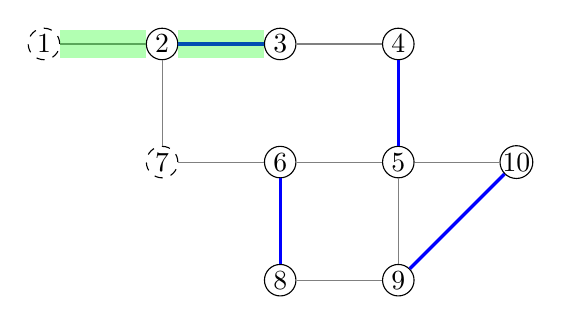
\begin{tikzpicture}
		\tikzstyle{Flower}	= [circle, fill=white, minimum size=4mm, inner sep=0pt]
		\tikzstyle{Vertex} 	= [circle, draw, solid,  fill=white, minimum size=4mm, inner sep=0pt]
		\tikzstyle{OUT}		= [fill = white]
		\tikzstyle{IN}		= [fill = black]
		\tikzstyle{Exposed}	= [dashed, OUT]
		\tikzstyle{MC}		= [very thick, blue]
		\tikzstyle{NM}		= [gray]
		
		\node (v1) at (0.0, 5.0) [Vertex][Exposed] {$1$};
		\node (v2) at (1.5, 5.0) [Vertex] {$2$};
		\node (v3) at (3.0, 5.0) [Vertex] {$3$};
		\node (v4) at (4.5, 5.0) [Vertex] {$4$};
		\node (v5) at (4.5, 3.5) [Vertex] {$5$};
		\node (v6) at (3.0, 3.5) [Vertex] {$6$};
		\node (v7) at (1.5, 3.5) [Vertex][Exposed] {$7$};
		\node (v8) at (3.0, 2.0) [Vertex] {$8$};
		\node (v9) at (4.5, 2.0) [Vertex] {$9$};
		\node (v10) at (6.0, 3.5) [Vertex] {$10$};
		
		\draw [-] (v1) to (v2) [NM];
		\draw [-] (v2) to (v3) [MC];
		\draw [-] (v2) to (v7) [NM];
		\draw [-] (v3) to (v4) [NM];
		\draw [-] (v4) to (v5) [MC];
		\draw [-] (v5) to (v6) [NM];
		\draw [-] (v5) to (v9) [NM];
		\draw [-] (v5) to (v10) [NM];
		\draw [-] (v6) to (v7) [NM];
		\draw [-] (v6) to (v8) [MC];
		\draw [-] (v8) to (v9) [NM];
		\draw [-] (v9) to (v10) [MC];
		
		\draw (v1) -- (v2) -- (v3) [line width=10pt, green, opacity=0.3];
	\end{tikzpicture}
	\end{center}

	If one vertex connected to the even vertex of the planted tree is in the matching, we can extend to a larger planted tree.
	
	\begin{center}
	\begin{tikzpicture}
		\tikzstyle{Flower}	= [circle, fill=white, minimum size=4mm, inner sep=0pt]
		\tikzstyle{Vertex} 	= [circle, draw, solid,  fill=white, minimum size=4mm, inner sep=0pt]
		\tikzstyle{OUT}		= [fill = white]
		\tikzstyle{IN}		= [fill = black]
		\tikzstyle{Exposed}	= [dashed, OUT]
		\tikzstyle{MC}		= [very thick, blue]
		\tikzstyle{NM}		= [gray]
		
		\node (v1) at (0.0, 5.0) [Vertex][Exposed][label=above:$even$] {$1$};
		\node (v2) at (1.5, 5.0) [Vertex][label=above:$odd$] {$2$};
		\node (v3) at (3.0, 5.0) [Vertex][label=above:$even$] {$3$};
		
		\draw [-] (v1) to (v2) [NM];
		\draw [-] (v2) to (v3) [MC];
		
		\draw (v1) -- (v2) -- (v3) [line width=10pt, green, opacity=0.3];
	\end{tikzpicture}
	\end{center}
	}
}

%---------------------slide--------------------%
\frame
{
	\frametitle{Examples}
	{\scriptsize
	A graph $G=(V,E)$ and a matching $M$.
	
	\begin{center}
	\begin{tikzpicture}
		\tikzstyle{Flower}	= [circle, fill=white, minimum size=4mm, inner sep=0pt]
		\tikzstyle{Vertex} 	= [circle, draw, solid,  fill=white, minimum size=4mm, inner sep=0pt]
		\tikzstyle{OUT}		= [fill = white]
		\tikzstyle{IN}		= [fill = black]
		\tikzstyle{Exposed}	= [dashed, OUT]
		\tikzstyle{MC}		= [very thick, blue]
		\tikzstyle{NM}		= [gray]
		
		\node (v1) at (0.0, 5.0) [Vertex][Exposed] {$1$};
		\node (v2) at (1.5, 5.0) [Vertex] {$2$};
		\node (v3) at (3.0, 5.0) [Vertex] {$3$};
		\node (v4) at (4.5, 5.0) [Vertex] {$4$};
		\node (v5) at (4.5, 3.5) [Vertex] {$5$};
		\node (v6) at (3.0, 3.5) [Vertex] {$6$};
		\node (v7) at (1.5, 3.5) [Vertex][Exposed] {$7$};
		\node (v8) at (3.0, 2.0) [Vertex] {$8$};
		\node (v9) at (4.5, 2.0) [Vertex] {$9$};
		\node (v10) at (6.0, 3.5) [Vertex] {$10$};
		
		\draw [-] (v1) to (v2) [NM];
		\draw [-] (v2) to (v3) [MC];
		\draw [-] (v2) to (v7) [NM];
		\draw [-] (v3) to (v4) [NM];
		\draw [-] (v4) to (v5) [MC];
		\draw [-] (v5) to (v6) [NM];
		\draw [-] (v5) to (v9) [NM];
		\draw [-] (v5) to (v10) [NM];
		\draw [-] (v6) to (v7) [NM];
		\draw [-] (v6) to (v8) [MC];
		\draw [-] (v8) to (v9) [NM];
		\draw [-] (v9) to (v10) [MC];
		
		\draw (v3) -- (v4) -- (v5) [line width=10pt, green, opacity=0.3];
	\end{tikzpicture}
	\end{center}

	Extend to a larger planted tree..
	
	\begin{center}
	\begin{tikzpicture}
		\tikzstyle{Flower}	= [circle, fill=white, minimum size=4mm, inner sep=0pt]
		\tikzstyle{Vertex} 	= [circle, draw, solid,  fill=white, minimum size=4mm, inner sep=0pt]
		\tikzstyle{OUT}		= [fill = white]
		\tikzstyle{IN}		= [fill = black]
		\tikzstyle{Exposed}	= [dashed, OUT]
		\tikzstyle{MC}		= [very thick, blue]
		\tikzstyle{NM}		= [gray]
		
		\node (v1) at (0.0, 5.0) [Vertex][Exposed][label=above:$even$] {$1$};
		\node (v2) at (1.5, 5.0) [Vertex][label=above:$odd$] {$2$};
		\node (v3) at (3.0, 5.0) [Vertex][label=above:$even$] {$3$};
		\node (v4) at (4.5, 5.0) [Vertex][label=above:$odd$] {$4$};
		\node (v5) at (6.0, 5.0) [Vertex][label=above:$even$] {$5$};
		
		\draw [-] (v1) to (v2) [NM];
		\draw [-] (v2) to (v3) [MC];
		\draw [-] (v3) to (v4) [NM];
		\draw [-] (v4) to (v5) [MC];
		
		\draw (v3) -- (v4) -- (v5) [line width=10pt, green, opacity=0.3];
	\end{tikzpicture}
	\end{center}
	}
}

%---------------------slide--------------------%
\frame
{
	\frametitle{Examples}
	{\scriptsize
	A graph $G=(V,E)$ and a matching $M$.
	
	\begin{center}
	\begin{tikzpicture}
		\tikzstyle{Flower}	= [circle, fill=white, minimum size=4mm, inner sep=0pt]
		\tikzstyle{Vertex} 	= [circle, draw, solid,  fill=white, minimum size=4mm, inner sep=0pt]
		\tikzstyle{OUT}		= [fill = white]
		\tikzstyle{IN}		= [fill = black]
		\tikzstyle{Exposed}	= [dashed, OUT]
		\tikzstyle{MC}		= [very thick, blue]
		\tikzstyle{NM}		= [gray]
		
		\node (v1) at (0.0, 5.0) [Vertex][Exposed] {$1$};
		\node (v2) at (1.5, 5.0) [Vertex] {$2$};
		\node (v3) at (3.0, 5.0) [Vertex] {$3$};
		\node (v4) at (4.5, 5.0) [Vertex] {$4$};
		\node (v5) at (4.5, 3.5) [Vertex] {$5$};
		\node (v6) at (3.0, 3.5) [Vertex] {$6$};
		\node (v7) at (1.5, 3.5) [Vertex][Exposed] {$7$};
		\node (v8) at (3.0, 2.0) [Vertex] {$8$};
		\node (v9) at (4.5, 2.0) [Vertex] {$9$};
		\node (v10) at (6.0, 3.5) [Vertex] {$10$};
		
		\draw [-] (v1) to (v2) [NM];
		\draw [-] (v2) to (v3) [MC];
		\draw [-] (v2) to (v7) [NM];
		\draw [-] (v3) to (v4) [NM];
		\draw [-] (v4) to (v5) [MC];
		\draw [-] (v5) to (v6) [NM];
		\draw [-] (v5) to (v9) [NM];
		\draw [-] (v5) to (v10) [NM];
		\draw [-] (v6) to (v7) [NM];
		\draw [-] (v6) to (v8) [MC];
		\draw [-] (v8) to (v9) [NM];
		\draw [-] (v9) to (v10) [MC];
		
		\draw (v5) -- (v10) -- (v9) [line width=10pt, green, opacity=0.3];
	\end{tikzpicture}
	\end{center}

	Extend to a larger planted tree....
	
	\begin{center}
	\begin{tikzpicture}
		\tikzstyle{Flower}	= [circle, fill=white, minimum size=4mm, inner sep=0pt]
		\tikzstyle{Vertex} 	= [circle, draw, solid,  fill=white, minimum size=4mm, inner sep=0pt]
		\tikzstyle{OUT}		= [fill = white]
		\tikzstyle{IN}		= [fill = black]
		\tikzstyle{Exposed}	= [dashed, OUT]
		\tikzstyle{MC}		= [very thick, blue]
		\tikzstyle{NM}		= [gray]
		
		\node (v1) at (0.0, 5.0) [Vertex][Exposed][label=above:$even$] {$1$};
		\node (v2) at (1.5, 5.0) [Vertex][label=above:$odd$] {$2$};
		\node (v3) at (3.0, 5.0) [Vertex][label=above:$even$] {$3$};
		\node (v4) at (4.5, 5.0) [Vertex][label=above:$odd$] {$4$};
		\node (v5) at (6.0, 5.0) [Vertex][label=above:$even$] {$5$};
		\node (v10) at (7.5, 5.0) [Vertex][label=above:$odd$] {$10$};
		\node (v9) at (8.0, 3.5) [Vertex][label=above:$even$] {$9$};
		
		\draw [-] (v1) to (v2) [NM];
		\draw [-] (v2) to (v3) [MC];
		\draw [-] (v3) to (v4) [NM];
		\draw [-] (v4) to (v5) [MC];
		\draw [-] (v5) to (v10) [NM];	
		\draw [-] (v9) to (v10) [MC];
		
		\draw (v5) -- (v10) -- (v9) [line width=10pt, green, opacity=0.3];
	\end{tikzpicture}
	\end{center}
	}
}

%---------------------slide--------------------%
\frame
{
	\frametitle{Examples}
	{\scriptsize
	A graph $G=(V,E)$ and a matching $M$.
	
	\begin{center}
	\begin{tikzpicture}
		\tikzstyle{Flower}	= [circle, fill=white, minimum size=4mm, inner sep=0pt]
		\tikzstyle{Vertex} 	= [circle, draw, solid,  fill=white, minimum size=4mm, inner sep=0pt]
		\tikzstyle{OUT}		= [fill = white]
		\tikzstyle{IN}		= [fill = black]
		\tikzstyle{Exposed}	= [dashed, OUT]
		\tikzstyle{MC}		= [very thick, blue]
		\tikzstyle{NM}		= [gray]
		
		\node (v1) at (0.0, 5.0) [Vertex][Exposed] {$1$};
		\node (v2) at (1.5, 5.0) [Vertex] {$2$};
		\node (v3) at (3.0, 5.0) [Vertex] {$3$};
		\node (v4) at (4.5, 5.0) [Vertex] {$4$};
		\node (v5) at (4.5, 3.5) [Vertex] {$5$};
		\node (v6) at (3.0, 3.5) [Vertex] {$6$};
		\node (v7) at (1.5, 3.5) [Vertex][Exposed] {$7$};
		\node (v8) at (3.0, 2.0) [Vertex] {$8$};
		\node (v9) at (4.5, 2.0) [Vertex] {$9$};
		\node (v10) at (6.0, 3.5) [Vertex] {$10$};
		
		\draw [-] (v1) to (v2) [NM];
		\draw [-] (v2) to (v3) [MC];
		\draw [-] (v2) to (v7) [NM];
		\draw [-] (v3) to (v4) [NM];
		\draw [-] (v4) to (v5) [MC];
		\draw [-] (v5) to (v6) [NM];
		\draw [-] (v5) to (v9) [NM];
		\draw [-] (v5) to (v10) [NM];
		\draw [-] (v6) to (v7) [NM];
		\draw [-] (v6) to (v8) [MC];
		\draw [-] (v8) to (v9) [NM];
		\draw [-] (v9) to (v10) [MC];
		
		\draw (v5) -- (v9) [line width=10pt, green, opacity=0.3];
	\end{tikzpicture}
	\end{center}

	Encounter an edge connecting two even vertices. Find a blossom!
	
	\begin{center}
	\begin{tikzpicture}
		\tikzstyle{Flower}	= [circle, fill=white, minimum size=4mm, inner sep=0pt]
		\tikzstyle{Vertex} 	= [circle, draw, solid,  fill=white, minimum size=4mm, inner sep=0pt]
		\tikzstyle{OUT}		= [fill = white]
		\tikzstyle{IN}		= [fill = black]
		\tikzstyle{Exposed}	= [dashed, OUT]
		\tikzstyle{MC}		= [very thick, blue]
		\tikzstyle{NM}		= [gray]
		
		\node (v1) at (0.0, 5.0) [Vertex][Exposed][label=above:$even$] {$1$};
		\node (v2) at (1.5, 5.0) [Vertex][label=above:$odd$] {$2$};
		\node (v3) at (3.0, 5.0) [Vertex][label=above:$even$] {$3$};
		\node (v4) at (4.5, 5.0) [Vertex][label=above:$odd$] {$4$};
		\node (v5) at (6.0, 5.0) [Vertex][label=above:$even$] {$5$};
		\node (v10) at (7.5, 5.0) [Vertex][label=above:$odd$] {$10$};
		\node (v9) at (8.0, 3.5) [Vertex][label=above:$even$] {$9$};
		
		\draw [-] (v1) to (v2) [NM];
		\draw [-] (v2) to (v3) [MC];
		\draw [-] (v3) to (v4) [NM];
		\draw [-] (v4) to (v5) [MC];
		\draw [-] (v5) to (v10) [NM];	
		\draw [-] (v9) to (v10) [MC];
		\draw [-] (v9) to (v5) [NM];
		
		\draw (v5) -- (v9) [line width=10pt, green, opacity=0.3];
	\end{tikzpicture}
	\end{center}
	}
}

%---------------------slide--------------------%
\frame
{
	\frametitle{Examples}

	{\scriptsize
	A graph $G=(V,E)$ and a matching $M$.
	
	\begin{center}
	\begin{tikzpicture}
		\tikzstyle{Flower}	= [circle, fill=white, minimum size=4mm, inner sep=0pt]
		\tikzstyle{Vertex} 	= [circle, draw, solid,  fill=white, minimum size=4mm, inner sep=0pt]
		\tikzstyle{OUT}		= [fill = white]
		\tikzstyle{IN}		= [fill = black]
		\tikzstyle{Exposed}	= [dashed, OUT]
		\tikzstyle{MC}		= [very thick, blue]
		\tikzstyle{NM}		= [gray]
		
		\node (v1) at (0.0, 5.0) [Vertex][Exposed] {$1$};
		\node (v2) at (1.5, 5.0) [Vertex] {$2$};
		\node (v3) at (3.0, 5.0) [Vertex] {$3$};
		\node (v4) at (4.5, 5.0) [Vertex] {$4$};
		\node (v5) at (4.5, 3.5) [Flower][label=below:\scriptsize{$(5,10,9)$}] {};
				\pgfplothandlerlineto
				\pgfplotfunction{\x}{0, 3, ..., 540}{
					\pgfpointxy     
					{-0.2 * cos(\x) * sin(5 / 3 * \x) + 4.5}
					{-0.2 * sin(\x) * sin(5 / 3 * \x) + 3.5}
				}
				\pgfusepath{stroke}
		\node (v6) at (3.0, 3.5) [Vertex] {$6$};
		\node (v7) at (1.5, 3.5) [Vertex][Exposed] {$7$};
		\node (v8) at (3.0, 2.0) [Vertex] {$8$};
		
		\draw [-] (v1) to (v2) [NM];
		\draw [-] (v2) to (v3) [MC];
		\draw [-] (v2) to (v7) [NM];
		\draw [-] (v3) to (v4) [NM];
		\draw [-] (v4) to (v5) [MC];
		\draw [-] (v5) to (v6) [NM];
		\draw [-] (v6) to (v7) [NM];
		\draw [-] (v6) to (v8) [MC];
		\draw [-] (v8) to (v5) [NM];
	\end{tikzpicture}
	\end{center}
	
	Shrink (5,10,9) into a single macro vertex.
	
	\begin{center}
	\begin{tikzpicture}
		\tikzstyle{Flower}	= [circle, fill=white, minimum size=4mm, inner sep=0pt]
		\tikzstyle{Vertex} 	= [circle, draw, solid,  fill=white, minimum size=4mm, inner sep=0pt]
		\tikzstyle{OUT}		= [fill = white]
		\tikzstyle{IN}		= [fill = black]
		\tikzstyle{Exposed}	= [dashed, OUT]
		\tikzstyle{MC}		= [very thick, blue]
		\tikzstyle{NM}		= [gray]
		
		\node (v1) at (0.0, 5.0) [Vertex][label=above:$even$][Exposed] {$1$};
		\node (v2) at (1.5, 5.0) [Vertex][label=above:$odd$] {$2$};
		\node (v3) at (3.0, 5.0) [Vertex][label=above:$even$] {$3$};
		\node (v4) at (4.5, 5.0) [Vertex][label=above:$odd$] {$4$};
		\node (v5) at (6.0, 5.0) [Flower][label=above:$even$][label=below:\scriptsize{$(5,10,9)$}] {};
			%\myflower.apply(6.0, 5.0, 0.3)	
				\pgfplothandlerlineto
				\pgfplotfunction{\x}{0, 3, ..., 540}{
					\pgfpointxy     
					{-0.2 * cos(\x) * sin(5 / 3 * \x) + 6.0}
					{-0.2 * sin(\x) * sin(5 / 3 * \x) + 5.0}
				}
				\pgfusepath{stroke}
						
		\draw [-] (v1) to (v2) [NM];
		\draw [-] (v2) to (v3) [MC];
		\draw [-] (v3) to (v4) [NM];
		\draw [-] (v4) to (v5) [MC];
	\end{tikzpicture}
	\end{center}
	}
}

%---------------------slide--------------------%
\frame
{
	\frametitle{Examples}

	{\scriptsize
	A graph $G=(V,E)$ and a matching $M$.
	
	\begin{center}
	\begin{tikzpicture}
		\tikzstyle{Flower}	= [circle, fill=white, minimum size=4mm, inner sep=0pt]
		\tikzstyle{Vertex} 	= [circle, draw, solid,  fill=white, minimum size=4mm, inner sep=0pt]
		\tikzstyle{OUT}		= [fill = white]
		\tikzstyle{IN}		= [fill = black]
		\tikzstyle{Exposed}	= [dashed, OUT]
		\tikzstyle{MC}		= [very thick, blue]
		\tikzstyle{NM}		= [gray]
		
		\node (v1) at (0.0, 5.0) [Vertex][Exposed] {$1$};
		\node (v2) at (1.5, 5.0) [Vertex] {$2$};
		\node (v3) at (3.0, 5.0) [Vertex] {$3$};
		\node (v4) at (4.5, 5.0) [Vertex] {$4$};
		\node (v5) at (4.5, 3.5) [Flower][label=below:\scriptsize{$(5,10,9)$}] {};
				\pgfplothandlerlineto
				\pgfplotfunction{\x}{0, 3, ..., 540}{
					\pgfpointxy     
					{-0.2 * cos(\x) * sin(5 / 3 * \x) + 4.5}
					{-0.2 * sin(\x) * sin(5 / 3 * \x) + 3.5}
				}
				\pgfusepath{stroke}
		\node (v6) at (3.0, 3.5) [Vertex] {$6$};
		\node (v7) at (1.5, 3.5) [Vertex][Exposed] {$7$};
		\node (v8) at (3.0, 2.0) [Vertex] {$8$};
		
		\draw [-] (v1) to (v2) [NM];
		\draw [-] (v2) to (v3) [MC];
		\draw [-] (v2) to (v7) [NM];
		\draw [-] (v3) to (v4) [NM];
		\draw [-] (v4) to (v5) [MC];
		\draw [-] (v5) to (v6) [NM];
		\draw [-] (v6) to (v7) [NM];
		\draw [-] (v6) to (v8) [MC];
		\draw [-] (v8) to (v5) [NM];
		
		\draw (v5) -- (v6) -- (v8) -- (v5) [line width=10pt, green, opacity=0.3];
	\end{tikzpicture}
	\end{center}
	
	Continue the search, and encounter the cycle (5,10,9)-6-8.
	
	\begin{center}
	\begin{tikzpicture}
		\tikzstyle{Flower}	= [circle, fill=white, minimum size=4mm, inner sep=0pt]
		\tikzstyle{Vertex} 	= [circle, draw, solid,  fill=white, minimum size=4mm, inner sep=0pt]
		\tikzstyle{OUT}		= [fill = white]
		\tikzstyle{IN}		= [fill = black]
		\tikzstyle{Exposed}	= [dashed, OUT]
		\tikzstyle{MC}		= [very thick, blue]
		\tikzstyle{NM}		= [gray]
		
		\node (v1) at (0.0, 5.0) [Vertex][label=above:$even$][Exposed] {$1$};
		\node (v2) at (1.5, 5.0) [Vertex][label=above:$odd$] {$2$};
		\node (v3) at (3.0, 5.0) [Vertex][label=above:$even$] {$3$};
		\node (v4) at (4.5, 5.0) [Vertex][label=above:$odd$] {$4$};
		\node (v5) at (6.0, 5.0) [Flower][label=above:$even$][label=below:\scriptsize{$5,10,9$}] {};
			%\myflower.apply(6.0, 5.0, 0.3)	
				\pgfplothandlerlineto
				\pgfplotfunction{\x}{0, 3, ..., 540}{
					\pgfpointxy     
					{-0.2 * cos(\x) * sin(5 / 3 * \x) + 6.0}
					{-0.2 * sin(\x) * sin(5 / 3 * \x) + 5.0}
				}
				\pgfusepath{stroke}
		\node (v6) at (7.5, 5.0) [Vertex][label=above:$odd$] {$6$};
		\node (v8) at (8.0, 3.5) [Vertex][label=above:$even$] {$8$};
		
		\draw [-] (v1) to (v2) [NM];
		\draw [-] (v2) to (v3) [MC];
		\draw [-] (v3) to (v4) [NM];
		\draw [-] (v4) to (v5) [MC];
		\draw [-] (v5) to (v6) [NM];
		\draw [-] (v5) to (v8) [NM];
		\draw [-] (v6) to (v8) [MC];
		
		\draw (v5) -- (v6) -- (v8) -- (v5) [line width=10pt, green, opacity=0.3];
	\end{tikzpicture}
	\end{center}
	}
}

%---------------------slide--------------------%
\frame
{
	\frametitle{Examples}

	{\scriptsize
	A graph $G=(V,E)$ and a matching $M$.
	
	\begin{center}
	\begin{tikzpicture}
		\tikzstyle{Flower}	= [circle, fill=white, minimum size=4mm, inner sep=0pt]
		\tikzstyle{Vertex} 	= [circle, draw, solid,  fill=white, minimum size=4mm, inner sep=0pt]
		\tikzstyle{OUT}		= [fill = white]
		\tikzstyle{IN}		= [fill = black]
		\tikzstyle{Exposed}	= [dashed, OUT]
		\tikzstyle{MC}		= [very thick, blue]
		\tikzstyle{NM}		= [gray]
		
		\node (v1) at (0.0, 5.0) [Vertex][Exposed] {$1$};
		\node (v2) at (1.5, 5.0) [Vertex] {$2$};
		\node (v3) at (3.0, 5.0) [Vertex] {$3$};
		\node (v4) at (4.5, 5.0) [Vertex] {$4$};
		\node (v5) at (4.5, 3.5) [Flower][label=below:\scriptsize{$(5,10,9),6,8$}] {};
				\pgfplothandlerlineto
				\pgfplotfunction{\x}{0, 3, ..., 540}{
					\pgfpointxy     
					{-0.2 * cos(\x) * sin(5 / 3 * \x) + 4.5}
					{-0.2 * sin(\x) * sin(5 / 3 * \x) + 3.5}
				}
				\pgfusepath{stroke}
		\node (v7) at (1.5, 3.5) [Vertex][Exposed] {$7$};
		
		\draw [-] (v1) to (v2) [NM];
		\draw [-] (v2) to (v3) [MC];
		\draw [-] (v2) to (v7) [NM];
		\draw [-] (v3) to (v4) [NM];
		\draw [-] (v4) to (v5) [MC];
		\draw [-] (v5) to (v7) [NM];
		
		\draw (v5) -- (v7) [line width=10pt, green, opacity=0.3];
	\end{tikzpicture}
	\end{center}
	
	Shrinke the blossom and encounter an exposed vertex 7.
	
	\begin{center}
	\begin{tikzpicture}
		\tikzstyle{Flower}	= [circle, fill=white, minimum size=4mm, inner sep=0pt]
		\tikzstyle{Vertex} 	= [circle, draw, solid,  fill=white, minimum size=4mm, inner sep=0pt]
		\tikzstyle{OUT}		= [fill = white]
		\tikzstyle{IN}		= [fill = black]
		\tikzstyle{Exposed}	= [dashed, OUT]
		\tikzstyle{MC}		= [very thick, blue]
		\tikzstyle{NM}		= [gray]
		
		\node (v1) at (0.0, 5.0) [Vertex][label=above:$even$][Exposed] {$1$};
		\node (v2) at (1.5, 5.0) [Vertex][label=above:$odd$] {$2$};
		\node (v3) at (3.0, 5.0) [Vertex][label=above:$even$] {$3$};
		\node (v4) at (4.5, 5.0) [Vertex][label=above:$odd$] {$4$};
		\node (v5) at (6.0, 5.0) [Flower][label=above:$even$][label=below:\scriptsize{$(5,10,9),6,8$}] {};
			%\myflower.apply(6.0, 5.0, 0.3)	
				\pgfplothandlerlineto
				\pgfplotfunction{\x}{0, 3, ..., 540}{
					\pgfpointxy     
					{-0.2 * cos(\x) * sin(5 / 3 * \x) + 6.0}
					{-0.2 * sin(\x) * sin(5 / 3 * \x) + 5.0}
				}
				\pgfusepath{stroke}
		\node (v7) at (7.5, 5.0) [Vertex][Exposed] {$7$};
		
		\draw [-] (v1) to (v2) [NM];
		\draw [-] (v2) to (v3) [MC];
		\draw [-] (v3) to (v4) [NM];
		\draw [-] (v4) to (v5) [MC];
		\draw [-] (v5) to (v7) [NM];
		
		\draw (v5) -- (v7) [line width=10pt, green, opacity=0.3];
	\end{tikzpicture}
	\end{center}
	}
}

%---------------------slide--------------------%
\frame
{
	\frametitle{Examples}

	{\scriptsize
	A graph $G=(V,E)$ and a matching $M$.
	
	\begin{center}
	\begin{tikzpicture}
		\tikzstyle{Flower}	= [circle, fill=white, minimum size=4mm, inner sep=0pt]
		\tikzstyle{Vertex} 	= [circle, draw, solid,  fill=white, minimum size=4mm, inner sep=0pt]
		\tikzstyle{OUT}		= [fill = white]
		\tikzstyle{IN}		= [fill = black]
		\tikzstyle{Exposed}	= [dashed, OUT]
		\tikzstyle{MC}		= [very thick, blue]
		\tikzstyle{NM}		= [gray]
		
		\node (v1) at (0.0, 5.0) [Vertex][Exposed] {$1$};
		\node (v2) at (1.5, 5.0) [Vertex] {$2$};
		\node (v3) at (3.0, 5.0) [Vertex] {$3$};
		\node (v4) at (4.5, 5.0) [Vertex] {$4$};
		\node (v5) at (4.5, 3.5) [Vertex] {$5$};
		\node (v6) at (3.0, 3.5) [Vertex] {$6$};
		\node (v7) at (1.5, 3.5) [Vertex][Exposed] {$7$};
		\node (v8) at (3.0, 2.0) [Vertex] {$8$};
		\node (v9) at (4.5, 2.0) [Vertex] {$9$};
		\node (v10) at (6.0, 3.5) [Vertex] {$10$};
		
		\draw [-] (v1) to (v2) [NM];
		\draw [-] (v2) to (v3) [MC];
		\draw [-] (v2) to (v7) [NM];
		\draw [-] (v3) to (v4) [NM];
		\draw [-] (v4) to (v5) [MC];
		\draw [-] (v5) to (v6) [NM];
		\draw [-] (v5) to (v9) [NM];
		\draw [-] (v5) to (v10) [NM];
		\draw [-] (v6) to (v7) [NM];
		\draw [-] (v6) to (v8) [MC];
		\draw [-] (v8) to (v9) [NM];
		\draw [-] (v9) to (v10) [MC];
		
		\draw (v1) -- (v2) -- (v3) -- (v4) -- (v5) -- (v10) -- (v9) -- (v8) -- (v6) -- (v7) [line width=10pt, red, opacity=0.3];
	\end{tikzpicture}
	\end{center}
		
	This is an augmenting tree and contains an augmenting path.
	
	\begin{center}
	\begin{tikzpicture}
		\tikzstyle{Flower}	= [circle, fill=white, minimum size=4mm, inner sep=0pt]
		\tikzstyle{Vertex} 	= [circle, draw, solid,  fill=white, minimum size=4mm, inner sep=0pt]
		\tikzstyle{OUT}		= [fill = white]
		\tikzstyle{IN}		= [fill = black]
		\tikzstyle{Exposed}	= [dashed, OUT]
		\tikzstyle{MC}		= [very thick, blue]
		\tikzstyle{NM}		= [gray]
		
		\node (v1) at (0.0, 5.0) [Vertex][label=above:$even$][Exposed] {$1$};
		\node (v2) at (1.5, 5.0) [Vertex][label=above:$odd$] {$2$};
		\node (v3) at (3.0, 5.0) [Vertex][label=above:$even$] {$3$};
		\node (v4) at (4.5, 5.0) [Vertex][label=above:$odd$] {$4$};
		\node (v5) at (6.0, 5.0) [Flower][label=above:$even$][label=below:\scriptsize{$(5,10,9),6,8$}] {};
			%\myflower.apply(6.0, 5.0, 0.3)	
				\pgfplothandlerlineto
				\pgfplotfunction{\x}{0, 3, ..., 540}{
					\pgfpointxy     
					{-0.2 * cos(\x) * sin(5 / 3 * \x) + 6.0}
					{-0.2 * sin(\x) * sin(5 / 3 * \x) + 5.0}
				}
				\pgfusepath{stroke}
		\node (v7) at (7.5, 5.0) [Vertex][Exposed] {$7$};
		
		\draw [-] (v1) to (v2) [NM];
		\draw [-] (v2) to (v3) [MC];
		\draw [-] (v3) to (v4) [NM];
		\draw [-] (v4) to (v5) [MC];
		\draw [-] (v5) to (v7) [NM];
	\end{tikzpicture}
	\end{center}
	}
}

%---------------------slide--------------------%
\frame{
	\frametitle{Examples}

	{

	Applying $M = M \oplus P$ yeilds following enlarged matching in the original graph.
	
	\begin{center}
	\begin{tikzpicture}
		\tikzstyle{Flower}	= [circle, fill=white, minimum size=4mm, inner sep=0pt]
		\tikzstyle{Vertex} 	= [circle, draw, solid,  fill=white, minimum size=4mm, inner sep=0pt]
		\tikzstyle{OUT}		= [fill = white]
		\tikzstyle{IN}		= [fill = black]
		\tikzstyle{Exposed}	= [dashed, OUT]
		\tikzstyle{MC}		= [very thick, blue]
		\tikzstyle{NM}		= [gray]
		
		\node (v1) at (0.0, 5.0) [Vertex] {$1$};
		\node (v2) at (1.5, 5.0) [Vertex] {$2$};
		\node (v3) at (3.0, 5.0) [Vertex] {$3$};
		\node (v4) at (4.5, 5.0) [Vertex] {$4$};
		\node (v5) at (4.5, 3.5) [Vertex] {$5$};
		\node (v6) at (3.0, 3.5) [Vertex] {$6$};
		\node (v7) at (1.5, 3.5) [Vertex] {$7$};
		\node (v8) at (3.0, 2.0) [Vertex] {$8$};
		\node (v9) at (4.5, 2.0) [Vertex] {$9$};
		\node (v10) at (6.0, 3.5) [Vertex] {$10$};
		
		\draw [-] (v1) to (v2) [MC];
		\draw [-] (v2) to (v3) [NM];
		\draw [-] (v2) to (v7) [NM];
		\draw [-] (v3) to (v4) [MC];
		\draw [-] (v4) to (v5) [NM];
		\draw [-] (v5) to (v6) [NM];
		\draw [-] (v5) to (v9) [NM];
		\draw [-] (v5) to (v10) [MC];
		\draw [-] (v6) to (v7) [MC];
		\draw [-] (v6) to (v8) [NM];
		\draw [-] (v8) to (v9) [MC];
		\draw [-] (v9) to (v10) [NM];
	\end{tikzpicture}
	\end{center}
	}
}

\frame
{
	\frametitle{Running time}
	\begin{itemize}
		\item At most $O(n)$ augmentations.
		\item Each augmentation will shrink at most $O(n)$ blossoms.
		\item Constructing the alternating tree takes at most $O(m)$.
		\item $\therefore O(n^{2}m)$
	\end{itemize}
}

%---------------------slide--------------------%
\section{Matching-duality theorem}
\frame
{
	\frametitle{Matching-duality theorem}

	\begin{block}{Linear programming duality theorem}
		If
		
		\begin{center}
		$x \geq 0, Ax \leq c$ 
		
		$y \geq 0, A^{T}y \geq b$
		\end{center}
		
		for given real vectors $b$ and $c$ and real matrix $A$, then for real vectors $x$ and $y$,
		
		\begin{center}
		$max_{x}(b,x) = min_{y}(c, y)$
		\end{center}
		
		if such extrema exist.
	\end{block}
}

%---------------------slide--------------------%
\frame
{
	\frametitle{Matching-duality theorem}	
	\begin{block}{K\"{o}nig theorem}
		In a bipartite graph, the maximum size of a matching is equal to the minimum size of a vertex cover.
	\end{block}

	\begin{center}
	\begin{tikzpicture}
		\tikzstyle{Flower}	= [circle, fill=white, minimum size=4mm, inner sep=0pt]
		\tikzstyle{Vertex} 	= [circle, draw, solid,  fill=white, minimum size=4mm, inner sep=0pt]
		\tikzstyle{OUT}		= [fill = white]
		\tikzstyle{IN}		= [fill = black]
		\tikzstyle{Exposed}	= [dashed, OUT]
		\tikzstyle{MC}		= [very thick, blue]
		\tikzstyle{NM}		= [gray]
		
		\node (v1) at (0.0, 1.0) [Vertex] {$1$};
		\node (v2) at (1.0, 1.0) [Vertex] {$2$};
		\node (v3) at (0.0, 0.0) [Vertex] {$3$};
		\node (v4) at (1.0, 0.0) [Vertex] {$4$};
		
		\draw [-] (v1) to (v3) [NM];
		\draw [-] (v2) to (v3) [NM];
		\draw [-] (v2) to (v4) [NM];
	\end{tikzpicture}
	\end{center}

	\begin{center}
	\begin{figure}[h]
		\hfill
		\centering
		\begin{minipage}[c]{.45\textwidth}
		\centering
		\begin{tikzpicture}
			\tikzstyle{Flower}	= [circle, fill=white, minimum size=4mm, inner sep=0pt]
			\tikzstyle{Vertex} 	= [circle, draw, solid,  fill=white, minimum size=4mm, inner sep=0pt]
			\tikzstyle{OUT}		= [fill = white]
			\tikzstyle{IN}		= [fill = black]
			\tikzstyle{Exposed}	= [dashed, OUT]
			\tikzstyle{MC}		= [very thick, blue]
			\tikzstyle{NM}		= [gray]
			
			\node (v1) at (0.0, 1.0) [Vertex] {$1$};
			\node (v2) at (1.0, 1.0) [Vertex] {$2$};
			\node (v3) at (0.0, 0.0) [Vertex] {$3$};
			\node (v4) at (1.0, 0.0) [Vertex] {$4$};
			
			\draw [-] (v1) to (v3) [MC];
			\draw [-] (v2) to (v3) [NM];
			\draw [-] (v2) to (v4) [MC];
		\end{tikzpicture}
		\end{minipage}
		\hfill
		\centering
		\begin{minipage}[c]{.45\textwidth}
		\centering
		\begin{tikzpicture}
			\tikzstyle{Flower}	= [circle, fill=white, minimum size=4mm, inner sep=0pt]
			\tikzstyle{Vertex} 	= [circle, draw, solid, fill=white, minimum size=4mm, inner sep=0pt]
			\tikzstyle{OUT}		= [fill = white]
			\tikzstyle{IN}		= [fill = red, opacity = 0.5]
			\tikzstyle{Exposed}	= [dashed, OUT]
			\tikzstyle{MC}		= [very thick, blue]
			\tikzstyle{NM}		= [gray]
			
			\node (v1) at (0.0, 1.0) [Vertex][IN] {$1$};
			\node (v2) at (1.0, 1.0) [Vertex][IN] {$2$};
			\node (v3) at (0.0, 0.0) [Vertex] {$3$};
			\node (v4) at (1.0, 0.0) [Vertex] {$4$};
			
			\draw [-] (v1) to (v3) [NM];
			\draw [-] (v2) to (v3) [NM];
			\draw [-] (v2) to (v4) [NM];
		\end{tikzpicture}
		\end{minipage}
		\hfill
	\end{figure}
	\end{center}
}

%---------------------slide--------------------%
\frame
{
	\frametitle{Matching-duality theorem}
	\begin{center}
	\begin{tikzpicture}
		\tikzstyle{Flower}	= [circle, fill=white, minimum size=4mm, inner sep=0pt]
		\tikzstyle{Vertex} 	= [circle, draw, solid,  fill=white, minimum size=4mm, inner sep=0pt]
		\tikzstyle{OUT}		= [fill = white]
		\tikzstyle{IN}		= [fill = black]
		\tikzstyle{Exposed}	= [dashed, OUT]
		\tikzstyle{MC}		= [very thick, blue]
		\tikzstyle{NM}		= [gray]
		
		\node (v1) at (0.0, 1.0) [Vertex] {$1$};
		\node (v2) at (1.0, 1.0) [Vertex] {$2$};
		\node (v3) at (0.0, 0.0) [Vertex] {$3$};
		\node (v4) at (1.0, 0.0) [Vertex] {$4$};
		
		\draw [-] (v1) to (v3) [NM];
		\draw [-] (v2) to (v3) [NM];
		\draw [-] (v2) to (v4) [NM];
	\end{tikzpicture}
	\end{center}
	
	\begin{center}
	\begin{figure}[h]
		\hfill
		\centering
		\begin{minipage}[c]{.45\textwidth}
		\centering
		\begin{block}{Maximum matching}
		maximize
		\begin{equation*}
		x_{13} + x_{23} + x_{24}
		\end{equation*}
		subject to
		\begin{equation*}
		\begin{array}{ccccccc}
	  	x_{13} &   &        &   &        & \leq & 1\\
		       &   & x_{23} & + & x_{24} & \leq & 1\\
		x_{13} & + & x_{23} &   &        & \leq & 1\\
		       &   &        &   & x_{24} & \leq & 1
	  	\end{array}
	  	\end{equation*}
		\end{block}
		\end{minipage}
		\hfill
		\centering
		\begin{minipage}[c]{.45\textwidth}
		\centering
		\begin{block}{Minimum cover}
		minimize
		\begin{equation*}
		x_{1} + x_{2} + x_{3} + x_{4}
		\end{equation*}
		subject to
		\begin{equation*}
		\begin{array}{cccccccc}
	  	x_{1}+ &        & x_{3} &       & \geq & 1\\
		       & x_{2}+ & x_{3} &       & \geq & 1\\
		       & x_{2}+ &       & x_{4} & \geq & 1\\
		       &        &       &       &      &  \\
	  	\end{array}
	  	\end{equation*}
		\end{block}
		\end{minipage}
		\hfill
	\end{figure}
	\end{center}
}

%---------------------slide--------------------%
\frame
{
	\frametitle{Matching-duality theorem}
	
	\begin{description}
	\item[Odd set cover] in a graph consists of a collection of vertices $S$ and odd-cardinality sets of vertices
$O_{1} , O_{2} , ..., O_{t}$ , disjoint from one another and from $S$, such that every edge of $G$ is either
incident with a vertex in $S$ or lies within an odd set $O_{j}$.
	\item[The capacity] of the odd-set cover is defined as: $|S| + \sum\limits_{j=1}^{t} \frac{|O_{j}| - 1}{2}$
	\end{description}
	
	\begin{figure}[htb]
	\centering
	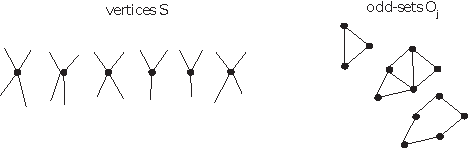
\includegraphics[width=0.8\textwidth]{figures/oddset.pdf}
	\end{figure}
}

%---------------------slide--------------------%
\frame
{
	\frametitle{Matching-duality theorem}
	
	\begin{block}{General K\"{o}nig theorem}
		If $M$ is a maximum matching and $C$ is a minimum odd-set cover then
		\begin{center}
		$|M| = capacity(C)$
		\end{center}
	\end{block}
	
	\begin{itemize}
	{
		\item Proof:
		
		\bigskip
		
		It is obvious that the capacity-sum of any odd-set cover in $G$ is at least as large as the cardinality of any matching in $G$, so we have only to prove the existence in $G$ of an odd-set cover and a matching for which the numbers are equal.
	}
	\end{itemize}
}

%---------------------slide--------------------%
\frame
{
	\frametitle{Matching-duality theorem}
	
	\begin{itemize}
	{
		\item Proof:

		\bigskip
				
		For a pertect matching $M$ with no exposed vertices
		
		\bigskip
		
		\begin{center}
		\begin{tikzpicture}
			\tikzstyle{Flower}	= [circle, fill=white, minimum size=4mm, inner sep=0pt]
			\tikzstyle{Vertex} 	= [circle, draw, solid,  fill=white, minimum size=4mm, inner sep=0pt]
			\tikzstyle{OUT}		= [fill = green, opacity = 0.5]
			\tikzstyle{IN}		= [fill = red, opacity = 0.5]
			\tikzstyle{Exposed}	= [dashed, OUT]
			\tikzstyle{MC}		= [very thick, blue]
			\tikzstyle{NM}		= [gray]
			
			\node (v1) at (0.0, 1.0) [Vertex][IN] {$1$};
			\node (v2) at (1.0, 1.0) [Vertex][OUT] {$2$};
			\node (v3) at (2.0, 1.0) [Vertex][OUT] {$3$};
			\node (v4) at (0.0, 0.0) [Vertex][OUT] {$4$};
			\node (v5) at (1.0, 0.0) [Vertex][OUT] {$5$};
			\node (v6) at (2.0, 0.0) [Vertex][OUT] {$6$};
			
			\draw [-] (v1) to (v4) [MC];
			\draw [-] (v2) to (v5) [MC];
			\draw [-] (v3) to (v6) [MC];
		\end{tikzpicture}
		\end{center}
		
	}
	\end{itemize}
}

%---------------------slide--------------------%
\frame
{
	\frametitle{Matching-duality theorem}
	
	\begin{itemize}
	{
		\item Proof:

		\bigskip
				
		For a graph which has a matching with one exposed vertices
		
		\bigskip
		
		\begin{center}
		\begin{tikzpicture}
			\tikzstyle{Flower}	= [circle, fill=white, minimum size=4mm, inner sep=0pt]
			\tikzstyle{Vertex} 	= [circle, draw, solid,  fill=white, minimum size=4mm, inner sep=0pt]
			\tikzstyle{OUT}		= [fill = green, opacity = 0.5]
			\tikzstyle{IN}		= [fill = red, opacity = 0.5]
			\tikzstyle{Exposed}	= [dashed, OUT]
			\tikzstyle{MC}		= [very thick, blue]
			\tikzstyle{NM}		= [gray]
			
			\node (v1) at (0.0, 1.0) [Vertex][Exposed][IN] {$1$};
			\node (v2) at (1.0, 1.0) [Vertex][IN] {$2$};
			\node (v3) at (2.0, 1.0) [Vertex][IN] {$3$};
			\node (v5) at (1.0, 0.0) [Vertex][IN] {$5$};
			\node (v6) at (2.0, 0.0) [Vertex][IN] {$6$};
			
			\draw [-] (v2) to (v5) [MC];
			\draw [-] (v3) to (v6) [MC];
		\end{tikzpicture}
		\end{center}
		
	}
	\end{itemize}
}

%---------------------slide--------------------%
\frame
{
	\frametitle{Matching-duality theorem}
	
	\begin{itemize}
	{
		\item Proof:

		\bigskip
				
		For a graph with more than one exposed vertex
		
		\bigskip
		
		\begin{center}
		\begin{tikzpicture}
			\tikzstyle{Flower}	= [circle, fill=white, minimum size=4mm, inner sep=0pt]
			\tikzstyle{Vertex} 	= [circle, draw, solid,  fill=white, minimum size=4mm, inner sep=0pt]
			\tikzstyle{OUT}		= [fill = green, opacity = 0.5]
			\tikzstyle{IN}		= [fill = red, opacity = 0.5]
			\tikzstyle{Exposed}	= [dashed]
			\tikzstyle{MC}		= [very thick, red]
			\tikzstyle{NM}		= [gray]
			
			\node (v1) at (0.0, 0.5) [Vertex] {$1$};
			\node (v2) at (1.0, 0.0) [Vertex] {$2$};
			\node (v3) at (1.0, 1.0) [Vertex] {$3$};
			\node (v4) at (2.0, 0.0) [Vertex][Exposed] {$4$};
			\node (v5) at (2.0, 1.0) [Vertex][Exposed] {$5$};
			\node (v6) at (0.0, 2.0) [Vertex] {$6$};
			\node (v7) at (-1.0, 2.0) [Vertex] {$7$};
			\node (v8) at (-1.0, 1.0) [Vertex] {$8$};
			\node (v9) at (2.0, 2.0) [Vertex] {$9$};
			\node (v10) at (1.0, 2.0) [Vertex] {$10$};
			
			\draw [-] (v1) to (v2) [MC];
			\draw [-] (v1) to (v3) [NM];
			\draw [-] (v2) to (v3) [NM];
			\draw [-] (v3) to (v4) [NM];
			\draw [-] (v3) to (v5) [NM];
			\draw [-] (v3) to (v6) [MC];
			\draw [-] (v6) to (v7) [NM];
			\draw [-] (v6) to (v8) [NM];
			\draw [-] (v7) to (v8) [MC];
			\draw [-] (v5) to (v9) [NM];
			\draw [-] (v5) to (v10) [NM];
			\draw [-] (v9) to (v10) [MC];
		\end{tikzpicture}
		\end{center}
		
	}
	\end{itemize}
}

%---------------------slide--------------------%
\frame
{
	\frametitle{Matching-duality theorem}
	
	\begin{itemize}
	{
		\item Proof:
		
		\begin{center}
		\begin{tikzpicture}
			\tikzstyle{Flower}	= [circle, fill=white, minimum size=4mm, inner sep=0pt]
			\tikzstyle{Vertex} 	= [circle, draw, solid,  fill=white, minimum size=4mm, inner sep=0pt]
			\tikzstyle{C1}		= [fill = green, opacity = 0.5]
			\tikzstyle{C2}		= [fill = blue, opacity = 0.5]
			\tikzstyle{Exposed}	= [dashed]
			\tikzstyle{MC}		= [very thick, red]
			\tikzstyle{NM}		= [gray]
			
			\node (v1) at (0.0, 0.5) [Vertex] {$1$};
			\node (v2) at (1.0, 0.0) [Vertex] {$2$};
			\node (v3) at (1.0, 1.0) [Vertex][C1] {$3$};
			\node (v4) at (2.0, 0.0) [Vertex][Exposed] {$4$};
			\node (v5) at (2.0, 1.0) [Vertex][Exposed] {$5$};
			\node (v6) at (0.0, 2.0) [Vertex][C2] {$6$};
			\node (v7) at (-1.0, 2.0) [Vertex][C2] {$7$};
			\node (v8) at (-1.0, 1.0) [Vertex][C2] {$8$};
			\node (v9) at (2.0, 2.0) [Vertex] {$9$};
			\node (v10) at (1.0, 2.0) [Vertex] {$10$};
			
			\draw [-] (v1) to (v2) [MC];
			\draw [-] (v1) to (v3) [NM];
			\draw [-] (v2) to (v3) [NM];
			\draw [-] (v3) to (v4) [NM];
			\draw [-] (v3) to (v5) [NM];
			\draw [-] (v3) to (v6) [MC];
			\draw [-] (v6) to (v7) [NM];
			\draw [-] (v6) to (v8) [NM];
			\draw [-] (v7) to (v8) [MC];
			\draw [-] (v5) to (v9) [NM];
			\draw [-] (v5) to (v10) [NM];
			\draw [-] (v9) to (v10) [MC];
			
			\draw (v4) -- (v3) -- (v6) -- (v7) -- (v8) -- (v6) [line width=10pt, red, opacity=0.3];
		\end{tikzpicture}
		\end{center}		
	}
	\end{itemize}
}

%---------------------slide--------------------%
\frame
{
	\frametitle{Matching-duality theorem}
	
	\begin{itemize}
	{
		\item Proof:
		
		\begin{center}
		\begin{tikzpicture}
			\tikzstyle{Flower}	= [circle, fill=white, minimum size=4mm, inner sep=0pt]
			\tikzstyle{Vertex} 	= [circle, draw, solid,  fill=white, minimum size=4mm, inner sep=0pt]
			\tikzstyle{C1}		= [fill = green, opacity = 0.5]
			\tikzstyle{C2}		= [fill = blue, opacity = 0.5]
			\tikzstyle{Exposed}	= [dashed]
			\tikzstyle{MC}		= [very thick, red]
			\tikzstyle{NM}		= [gray]
			
			\node (v1) at (0.0, 0.5) [Vertex] {$1$};
			\node (v2) at (1.0, 0.0) [Vertex] {$2$};
			\node (v3) at (1.0, 1.0) [Vertex][C1] {$3$};
			\node (v4) at (2.0, 0.0) [Vertex][Exposed] {$4$};
			\node (v5) at (2.0, 1.0) [Vertex][Exposed] {$5$};
			\node (v6) at (0.0, 2.0) [Vertex][C2] {$6$};
			\node (v7) at (-1.0, 2.0) [Vertex][C2] {$7$};
			\node (v8) at (-1.0, 1.0) [Vertex][C2] {$8$};
			\node (v9) at (2.0, 2.0) [Vertex] {$9$};
			\node (v10) at (1.0, 2.0) [Vertex] {$10$};
			
			\draw [-] (v1) to (v2) [MC];
			\draw [-] (v1) to (v3) [NM];
			\draw [-] (v2) to (v3) [NM];
			\draw [-] (v3) to (v4) [NM];
			\draw [-] (v3) to (v5) [NM];
			\draw [-] (v3) to (v6) [MC];
			\draw [-] (v6) to (v7) [NM];
			\draw [-] (v6) to (v8) [NM];
			\draw [-] (v7) to (v8) [MC];
			\draw [-] (v5) to (v9) [NM];
			\draw [-] (v5) to (v10) [NM];
			\draw [-] (v9) to (v10) [MC];
			
			\draw (v4) -- (v3) -- (v6) -- (v7) -- (v8) -- (v6) [line width=10pt, red, opacity=0.3];
		\end{tikzpicture}
		\end{center}	
		
		\bigskip
		
		\begin{center}
		\begin{tikzpicture}
			\tikzstyle{Flower}	= [circle, fill=white, minimum size=4mm, inner sep=0pt]
			\tikzstyle{Vertex} 	= [circle, draw, solid,  fill=white, minimum size=4mm, inner sep=0pt]
			\tikzstyle{C1}		= [fill = green, opacity = 0.5]
			\tikzstyle{C2}		= [fill = blue, opacity = 0.5]
			\tikzstyle{Exposed}	= [dashed]
			\tikzstyle{MC}		= [very thick, red]
			\tikzstyle{NM}		= [gray]
			
			\node (v1) at (0.0, 0.5) [Vertex][C1] {$1$};
			\node (v2) at (1.0, 0.0) [Vertex] {$2$};
			\node (v3) at (1.0, 1.0) [Vertex] {$3$};
			\node (v4) at (2.0, 0.0) [Vertex][Exposed] {$4$};
			\node (v5) at (2.0, 1.0) [Vertex][Exposed][C2]  {$5$};
			\node (v6) at (0.0, 2.0) [Vertex] {$6$};
			\node (v7) at (-1.0, 2.0) [Vertex] {$7$};
			\node (v8) at (-1.0, 1.0) [Vertex] {$8$};
			\node (v9) at (2.0, 2.0) [Vertex][C2]  {$9$};
			\node (v10) at (1.0, 2.0) [Vertex][C2]  {$10$};
			
			\draw [-] (v1) to (v2) [MC];
			\draw [-] (v3) to (v4) [NM];
			\draw [-] (v3) to (v6) [MC];
			\draw [-] (v6) to (v7) [NM];
			\draw [-] (v6) to (v8) [NM];
			\draw [-] (v7) to (v8) [MC];
			\draw [-] (v5) to (v9) [NM];
			\draw [-] (v5) to (v10) [NM];
			\draw [-] (v9) to (v10) [MC];
			
			\draw (v1) -- (v2) [line width=10pt, red, opacity=0.3];
			\draw (v5) -- (v9) -- (v10) -- (v5) [line width=10pt, red, opacity=0.3];
		\end{tikzpicture}
		\end{center}
	}
	\end{itemize}
}

\end{document}
